\documentclass[]{myclass}
\usepackage[cp1250]{inputenc}
\usepackage[OT4]{fontenc}
\usepackage{hyperref}
\usepackage[table,xcdraw]{xcolor}
\usepackage{multirow}
\usepackage{subfig}
\usepackage{float}
\usepackage{amsfonts}
\usepackage{pdfpages}
\usepackage{listings}
\usepackage[english]{babel}
\usepackage{titling}
\usepackage{tocbibind}
\definecolor{mygreen}{rgb}{0,0.6,0}
\lstset {
basicstyle=\small,
breaklines=true,
commentstyle=\color{mygreen},
keywordstyle=\color{blue},
language=C,
linewidth=\textwidth
}
\linespread{1}

\author{Marcin Aftowicz}
\title{Hardware Test and fault diagnosis based on extended FEC functions  in wireless communication systems}
\mysupervisor{Prof. Dr.-Ing. H. T. Vierhaus \and Ing. Petr Pfeifer, MSc, MBA, Ph.D.}
\myyear{2018}

\begin{document}
\selectlanguage{english}
\bibliographystyle{plplain}

% Front matter **************************************
\frontmatter
\pagestyle{empty}%
\maketitle  \cleardoublepage

\pagenumbering{Roman}
\phantomsection
\addcontentsline{toc}{chapter}{Statutory declaration}

{\noindent}STATUTORY DECLARATION\\

I declare that I have authored this thesis independently, that I have not used other than the declared 
sources  /  resources,  and  that  I  have  explicitly  marked  all  material  which  has  been  quoted  either  
literally or by content from the used sources. \\
\par\vspace{15mm}\par

Marcin Aftowicz \hfill Date \hspace{2cm}

   \cleardoublepage

\pagestyle{ppfcmthesis}
\phantomsection
\addcontentsline{toc}{chapter}{Abstract}
\begin{abstract}
Wireless communication is more and more commonly used in highly unfavorable environments. Nowadays it's not only cellular communication, but also communication within cities, industrial production facilities and other short distance, real-time applications. Such systems have significant demand on safety whilst being vastly exposed not only to signal interferences, multi-path signal propagation and fading effects, but also to transient and permanent faults in hardware. While communication errors are covered by increasingly effective error correcting codes, the permanent faults in hardware still pose a threat to dependability. Since the communication systems consist of digital, analog and mixed-signal circuitry, the diagnostic test to uncover permanent faults happens in every module separately. The test extensions have to be built in during the development process, which is difficult in systems with no access to the internal structure of some IPs, e.g. due to patent protection. The following thesis describes the implementation of a diagnostic test, while treating the communication system as a whole and using the forward error correction units for error position determination.
\vfill


 \noindent Marcin Aftowicz m.j.aftowicz@gmail.com \newline


\end{abstract}    \cleardoublepage

\listoffigures  \cleardoublepage
\listoftables   \cleardoublepage

\hypersetup{
    linkcolor={blue!70!black},
    citecolor={blue!70!black},
    urlcolor={blue!70!black}
}
\tableofcontents \cleardoublepage

% Main matter **************************************
\mainmatter
 
%Define necessary functions for diagnostic tests	   
%Define encoder/decoder extensions	   
%Implement extensions on FPGAs	   
%Develop diagnostic test interface software to control / set optional parameters and record results	   
%Implement into FPGA an experimental set-up	   
%Conduct measurements on examples

%das Block-Diagramm zu ParSec zeigen
%zeigen wie der Baseband-Prozessor aufgebaut ist (digital-analog), so dass ein direkter interner Test mit bekannten "digitalen" Verfahren schwierig ist.
%vorstellen, dass man bei einem System wie in ParSec ohne FEC nicht auskommt.
%Zeigen, dass FEC-Komponenten partiell eigene Fehler korrigieren.
%zeigen (Petr!) wie man bei den FEC-Komponenten Selbsttest-Funktionen einbauen kann.

%=============================================================
\chapter{Introduction and motivation} \label{ch:introduction}
Wireless signal transmission and data storage are getting more and more exposed to faults. For many years scientists have investigated the problem and suggested 
The wireless communication system consist of the source encoder and decoder, which get rid of the useless redundancy maximizing the information throughput, followed by cryptographic encoder and decoder, to make the information secret, followed by the channel encoder and decoder for error detection and correction. Then the information is processed by a baseband processor and is sent over radio. 
When using hash functions even a single bit flip leads to totally different results.
%=============================================================

\chapter{Coding theory} \label{ch:coding}
In the year 1948 Shannon published a landmarking article about the theory of communication, \cite{article:shannon} where he showed that with certain information encoding the errors induced by noisy channel can be significantly reduced. The data transmission and data storage can be both treated as equivalent in the digital data transmission path model shown in \hyperref[fig:data_path]{Figure~\ref*{fig:data_path}}. They both transfer data from the source to sink and they are both exposed to noise during the process.\\

\section{Channel coding} label{sec:channel}
In relation to \hyperref[fig:data_path]{Figure~\ref*{fig:data_path}} the purpose of the channel encoder is to transform the information sequence $u$, produced by the source encoder, into a discrete sequence called $code word$

\begin  {figure}  [h]
\centering
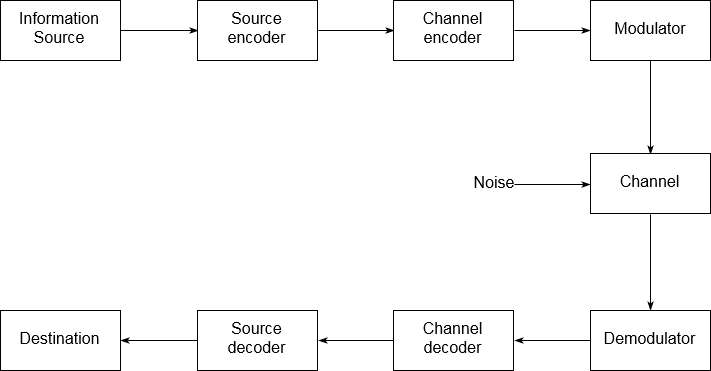
\includegraphics[width=0.65\textwidth]{figures/Data_transmission_path.png}
\caption{Block diagram of a typical data transmission system \cite{book:1983}}
\label{fig:data_path}
\end {figure}

While the source encoder strips the source output of redundant bits, maximizing the information throughput; the channel encoder adds useful bits to allow reliable data transfer, therefore the channel encoder will be the subject of further investigation. 

%=============================================================
\section{Model systemu} \label{sec:model}

%Zdecydowano si� na stworzenie systemu wbudowanego, kt�ry spe�ni wymagania przedstawione w \hyperref[sec:analiza]{Sekcji~\ref*{sec:analiza}: Analiza problemu}. W celu zbierania danych potrzebny jest osobny uk�ad, kt�ry b�dzie odpowiedzialny za konkretn� grup� czujnik�w, dalej zwany jednostk� pomiarow� (HUB). Pozwala to na wi�ksz� elastyczno�� podczas doboru czujnik�w oraz protoko��w komunikacyjnych. Niweluje to r�wnie� problem przesy�u sygna�u z czujnik�w na du�e odleg�o�ci do jednego centralnego urz�dzenia, zmniejszaj�c r�wnie� ilo�� przewod�w w poje�dzie. Centralne urz�dzenie jest dalej zwane g��wnym komputerem pok�adowym. Komputer pok�adowy ma za zadanie zebranie danych, wy�wietlanie ich oraz archiwizacj�. Komunikacja mi�dzy jednostkami pomiarowymi, a g��wnym komputerem pok�adowym musi by� odporna na zak��cenia, gdy� odleg�o�ci mi�dzy tymi urz�dzeniami mog� by� znaczne, a dowolno�� u�o�enia przewod�w ograniczona przez konstrukcj� pojazdu. Komunikacja musi zapewni� wszystkim jednostkom pomiarowym czas na wys�anie wiadomo�ci, a komputerowi pok�adowemu na archiwizacj� i przesy� do interfejsu u�ytkownika. Dlatego komunikacja ta musi by� szybka i niezawodna. Wybrano do tego celu platform� sprz�tow� z wbudowanym kontrolerem magistrali Controller Area Network ($CAN$), kt�ry autonomicznie wykonuje cz�� operacji, odci��aj�c jednostk� centraln�. W celu archiwizacji danych u�yto karty SD, kt�ra zapewnia mo�liwo�� obs�ugi zar�wno przez wbudowany system, jak i przez komputer osobisty. Umo�liwia r�wnie� du�e pr�dko�ci zapisu danych, a dzi�ki wbudowanemu kontrolerowi dost�pu do pami�ci ($DMA$), odci��a jednostk� centraln�. Do komunikacji bezprzewodowej wybrano modu� radiowy XBee, kt�ry umo�liwia komunikacj� na du�e odleg�o�ci, co pozwala utrzyma� komunikacj� podczas przejazd�w pojazdu na d�ugich trasach. Jest obs�ugiwany przez zintegrowany uk�ad $UART$.
\begin  {figure} [h] 
\centering
\includegraphics[width=0.75\textwidth]{figures/model1.JPG}
\caption{Model systemu pomiarowego}
\label{fig:model}
\end {figure}

\subsection{Prototyp}
We wczesnych fazach projektu stworzono prototyp urz�dzenia, w kt�rym zaimplementowano obs�ug� karty SD przez protok� $SPI$. Rozwi�zanie sprawdza�o si� dla uproszczonej sieci $CAN$, w kt�rej obs�uga magistrali by�a jedynym zadaniem procesora. Ramki na magistrali $CAN$ by�y przesy�ane w losowych odst�pach czasowych, bez u�ycia filtr�w akceptacyjnych. Nast�powa�a wymiana informacji mi�dzy jedn� jednostk� pomiarow�, a g��wnym komputerem (w obie strony). Kolejny komunikat by� wysy�any po przetworzeniu poprzedniego. Obs�ugiwano jeden kana� przetwornika, upraszczaj�c problem adresowania (istnia� tylko jeden identyfikator w ca�ej sieci). Projekt ewoluowa� i zosta� udoskonalony przybieraj�c dzisiejsz� form�. Planowane s� dalsze prace nad optymalizacj� jego dzia�ania.

\section{G��wny komputer pok�adowy}
\textit{Autor: Marcin Aftowicz}\\ \\

%Komputer pok�adowy sk�ada si� z dw�ch element�w: p�ytki ewaluacyjnej STM32\-F4\-Dis\-co\-ve\-ry~\cite{manual:discovery} oraz nak�adki rozszerzaj�cej jej mo�liwo�ci.  Oprogramowanie komputera pok�adowego stanowi zestaw funkcji oraz projekt�w, w kt�rych testowane s� poszczeg�lne podzespo�y oraz ich wzajemna integracja. Fragmenty kodu programu umieszczone s� w niniejszym rozdziale, w odpowiadaj�cych im sekcjach. W ramach tworzenia projektu powsta� projekt p�ytki drukowanej wraz z modelem $3D$ aby zilustrowa�  wygl�d nak�adki do modu�u Discovery. Model przedstawiono na \hyperref[fig:3D]{Rysnuku~\ref*{fig:3D}}.

\subsection{Mikrokontroler} \label{sec:sub:mcu}
G��wnym podzespo�em komputera pok�adowego jest mikrokontroler serii STM32F4. Nazwa serii reprezentuje kolejno nazw� producenta - STMicroelectronics, wielko�� pojedynczego rejestru - 32 bity oraz wersj� rdzenia - Cortex�-M4 CPU firmy ARM \cite{article:discovery}\cite{manual:discovery}. Jest to podrodzina rdzeni zoptymalizowana pod k�tem minimalizacji ceny przy zachowaniu du�ej wydajno�ci, przeznaczona do zastosowa� konsumenckich i przemys�owych \cite{book:paprocki}. Powodem wyboru tej platformy sprz�towej jest spe�nienie przez ni� wszystkich za�o�e� projektu odno�nie jednostki steruj�cej oraz posiadanych uk�ad�w peryferyjnych \cite{manual:stm32f4d}. Uk�ad musi 
\begin{itemize}
\item by� szybki - 168 MHz,
\item by� niezawodny - dwa timery typu watchdog,
\item posiada� rozszerzenie $SDIO$ do obs�ugi kart SD\\
(\hyperref[sec:sd]{Sekcja~\ref*{sec:sd}: Archiwizacja danych}),
\item posiada� magistral� $CAN$ do komunikacji z uk�adami pomocniczymi\\ (\hyperref[sec:can]{Sekcja~\ref*{sec:can}: G��wna magistrala komunikacyjna}),
\item posiada� kontroler $UART$ do komunikacji z nadajnikiem XBee\\
(\hyperref[sec:xbee]{Sekcja~\ref*{sec:xbee}: Komunikacja bezprzewodowa})
\item by� �atwy w  programowaniu, co umo�liwi�a rozbudowana biblioteka dostarczana przez producenta,
\end{itemize}

P�ytka STM32 Discovery to zestaw ewaluacyjny pomagaj�cy zrozumie� dzia�anie procesor�w 32-bitowych serii F4. Posiada procesor STM32F407VG. Zastosowanie nak�adki rozszerzaj�cej funkcjonalno�� Discovery pozwala znacznie u�atwi� proces projektowania skracaj�c go znacznie. Zestaw posiada wbudowany programator ST-LINK/V2 z interfejsem USB, s�u��cy do programowania i debugowania programu. Dodatkowo posiada port USB OTG, akcelerometr, mikrofon, diody oraz przyciski. Wszystkie uk�ady peryferyjne maj� swoje wyprowadzenia i w �atwy spos�b mo�na stworzy� prototypowy system przy u�yciu przewod�w i p�ytki stykowej. Dodatkowo firma STMicroelectronics udost�pnia przyk�adowe programy oraz biblioteki do u�ytku na Discovery~\cite{manual:discovery}.

\subsection{Obs�uga magistrali CAN}
G��wn� magistral� komunikacyjn� w systemie jest Controller Area Network opisany w \hyperref[sec:can]{Sekcji~\ref*{sec:can}: G��wna magistrala komunikacyjna}. Implementacja komunikacji przy wykorzystaniu tej magistrali by�a g��wnym celem projektu. Komunikacja mo�liwa jest dzi�ki kontrolerowi magistrali $CAN$ zintegrowanemu w mikrokontrolerze. Posiada on trzy skrzynki nadawcze i dwie odbiorcze, kt�re mieszcz� po trzy wiadomo�ci. Dodatkowo wyposa�ony jest w bank filtr�w akceptacyjnych, kt�re mo�na dowolnie przypisa� do dw�ch interfejs�w $CAN$, po 14 do ka�dego. Odbi�r wiadomo�ci odbywa si� automatycznie i jest realizowany sprz�towo, podobnie jak wst�pna selekcja nadchodz�cych komunikat�w. Filtry odci��aj� procesor, sortuj�c wiadomo�ci.~\cite{manual:stm32f4}.\\
Dzi�ki u�yciu protoko�u $CAN$ system ma mo�liwo�� odczytywania danych ze sterownika silnika $ECU$ serii PE3~\cite{manual:ecu}, kt�ry wysy�a wiadomo�ci przy u�yciu standardu bazuj�cego na SAE J1939~\cite{sae:j1939}. Dok�adna znajomo�� standardu SAE J1939 nie jest potrzebna w celu zbudowania systemu mog�cego si� komunikowa� ze sterownikiem. Producent do��cza not� katalogow�~\cite{manual:ecu}, w kt�rej opisane s� wszystkie mo�liwe komunikaty, kt�re sterownik wysy�a. 

\subsubsection{Przestrze� adresowa CAN} \label{ssec:adresowanie}
Ka�dy identyfikator w standardzie SAE J1939, u�ywanym w sterowniku $ECU$, oparty jest na rozszerzonej wersji standardu $CAN$ i posiada 29 bit�w. Ka�da wiadomo��, posiadaj�ca w�asny identyfikator, niesie ze sob� 7 lub 8 bajt�w danych, czyli maksymaln� ilo�� przewidzian� przez standard $CAN$. Producent sterownika $ECU$ do��cza instrukcj� s�u��c� do dekodowania ramki, w celu uzyskania pojedynczych informacji zawartych w 8-bajtowym komunikacie~\cite{manual:ecu}. Na podstawie identyfikator�w u�ywanych przez $ECU$ zbudowano system identyfikator�w wyst�puj�cych w systemie. Pomimo i� identyfikator przypisany jest do wiadomo�ci, a nie do urz�dzenia, utworzono system filtr�w, kt�ry jednoznacznie okre�la, kt�ry w�ze� magistrali nades�a� wiadomo��. Format identyfikatora przedstawiono na \hyperref[fig:identyfikatory]{Rysunku~\ref*{fig:identyfikatory}} i jest to przyk�ad identyfikatora u�ywanego przez sterownik silnika $ECU$.

\begin  {figure} [h] 
\centering
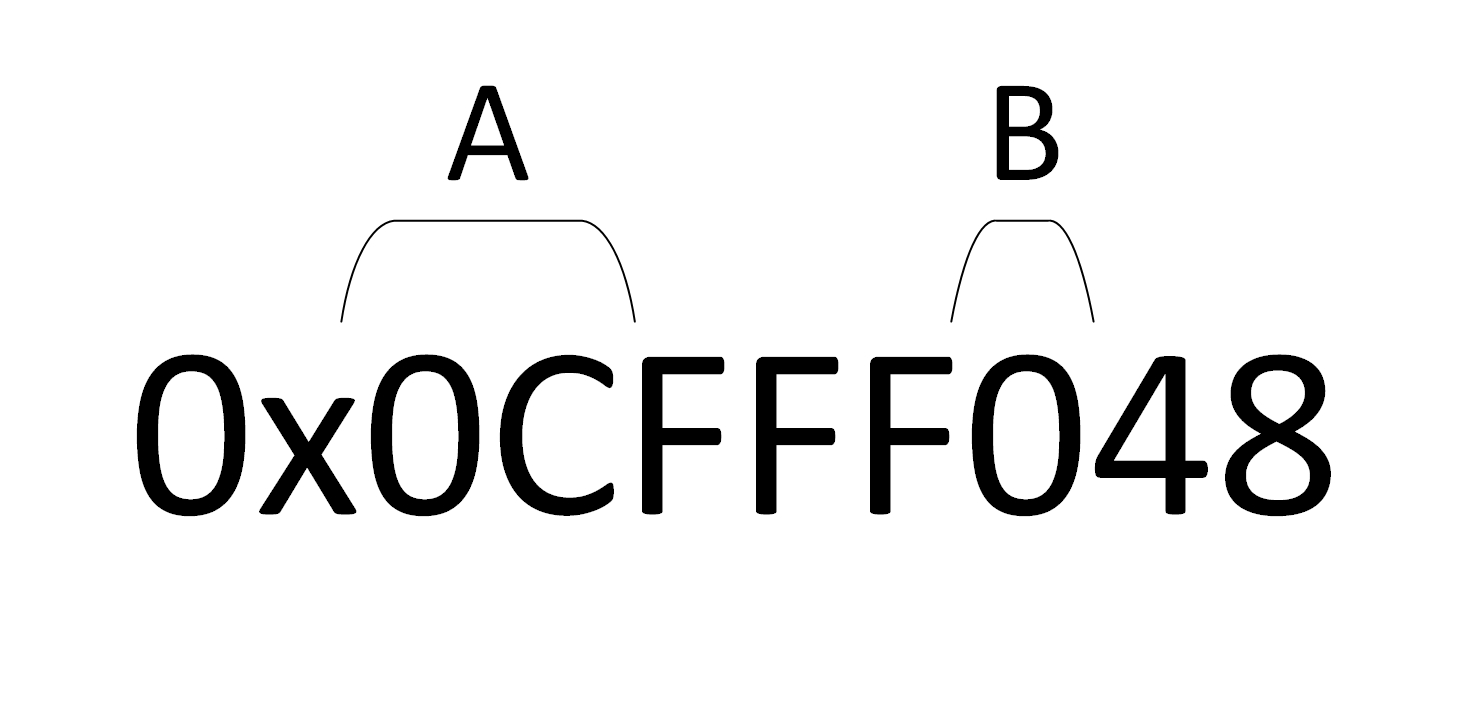
\includegraphics[width=0.3\textwidth]{figures/Adress.JPG}
\caption{Budowa identyfikatora $CAN$}
\label{fig:identyfikatory}
\end {figure}

\begin{itemize}
\item Segment A odpowiedzialny jest za adres urz�dzenia i przybiera warto�ci od 0x06 do 0x12. Zakres ten umo�liwia  obs�ug� do 13 pod��czonych urz�dze� (HUB 0 - HUB 12). Jest to niewielka ilo��, bior�c pod uwag� mo�liwo�ci jakie oferuje standard $CAN$. Nie zak�ada si� jednak wi�kszej potrzeby. Adresowanie zosta�o tak skonstruowane, aby identyfikator $ECU$, kt�rego segment A wynosi 0x0C znajdowa� si� w �rodku zakresu (HUB 6). Pami�taj�c, �e identyfikator wiadomo�ci jest jednocze�nie jej priorytetem, takie roz�o�enie identyfikator�w pozwala z du�� dowolno�ci� ustawia� system priorytet�w pomi�dzy w�z�ami.\\
\noindent \begin{minipage}{\textwidth}
\begin{lstlisting}[captionpos=b, belowcaptionskip=8pt, caption=Lista mo�liwych identyfikator�w $CAN$, label=listing:identyfikatory]
#define	CAN_ID_HUB12	0x12FFF048 // 1 0010 *** Lowest Priority ***
#define	CAN_ID_HUB11	0x11FFF048 // 1 0001
#define	CAN_ID_HUB10	0x10FFF048 // 1 0000
#define	CAN_ID_HUB9	0x0FFFF048 // 0 1111
#define	CAN_ID_HUB8	0x0EFFF048 // 0 1110
#define	CAN_ID_HUB7	0x0DFFF048 // 0 1101
#define	CAN_ID_HUB6	0x0CFFF048 // 0 1100 ECU
#define	CAN_ID_HUB5	0x0BFFF048 // 0 1011 
#define	CAN_ID_HUB4	0x0AFFF048 // 0 1010 
#define	CAN_ID_HUB3	0x09FFF048 // 0 1001 
#define	CAN_ID_HUB2	0x08FFF048 // 0 1000 
#define	CAN_ID_HUB1	0x07FFF048 // 0 0111 
#define	CAN_ID_HUB0	0x06FFF048 // 0 0110 *** Highest Priority ***
\end{lstlisting}
\end{minipage}
\item Segment B odpowiedzialny jest za rozr�nienie, co zawiera komunikat. W sterowniku $ECU$ s� to warto�ci od 0x0 do 0x6. Aby zdekodowa� komunikat nadawany przez $ECU$, nale�y odnie�� si� do noty katalogowej~\cite{manual:ecu}. Pozosta�e w�z�y przyjmuj� w segmencie B warto�ci od 0x0 do 0xA. Ka�dy identyfikator skojarzony jest z kana�em przetwornika anlogowo-cyfrowego, kt�ry jest cz�ci� architektury jednostki pomiarowej. Przetworniki posiadaj� rozdzielczo�� 12 bit�w, dzi�ki czemu wystarcz� dwa bajty danych na przes�anie wiadomo�ci. Ka�da wiadomo�� posiada sw�j identyfikator co sprawia, �e wynikiem filtrowania wiadomo�ci b�dzie dok�adna informacja o stanie konkretnego wej�cia analogowego jednostki pomiarowej.
\end{itemize}
Adresowanie wiadomo�ci przedstawiono na \hyperref[fig:adresowanie]{Rysunku~\ref*{fig:adresowanie}}. Nieu�ywane bajty w identyfikatorze stanowi� mo�liwo�� do rozszerzenia funkcjonalno�ci systemu.

\begin  {figure} [h] 
\centering
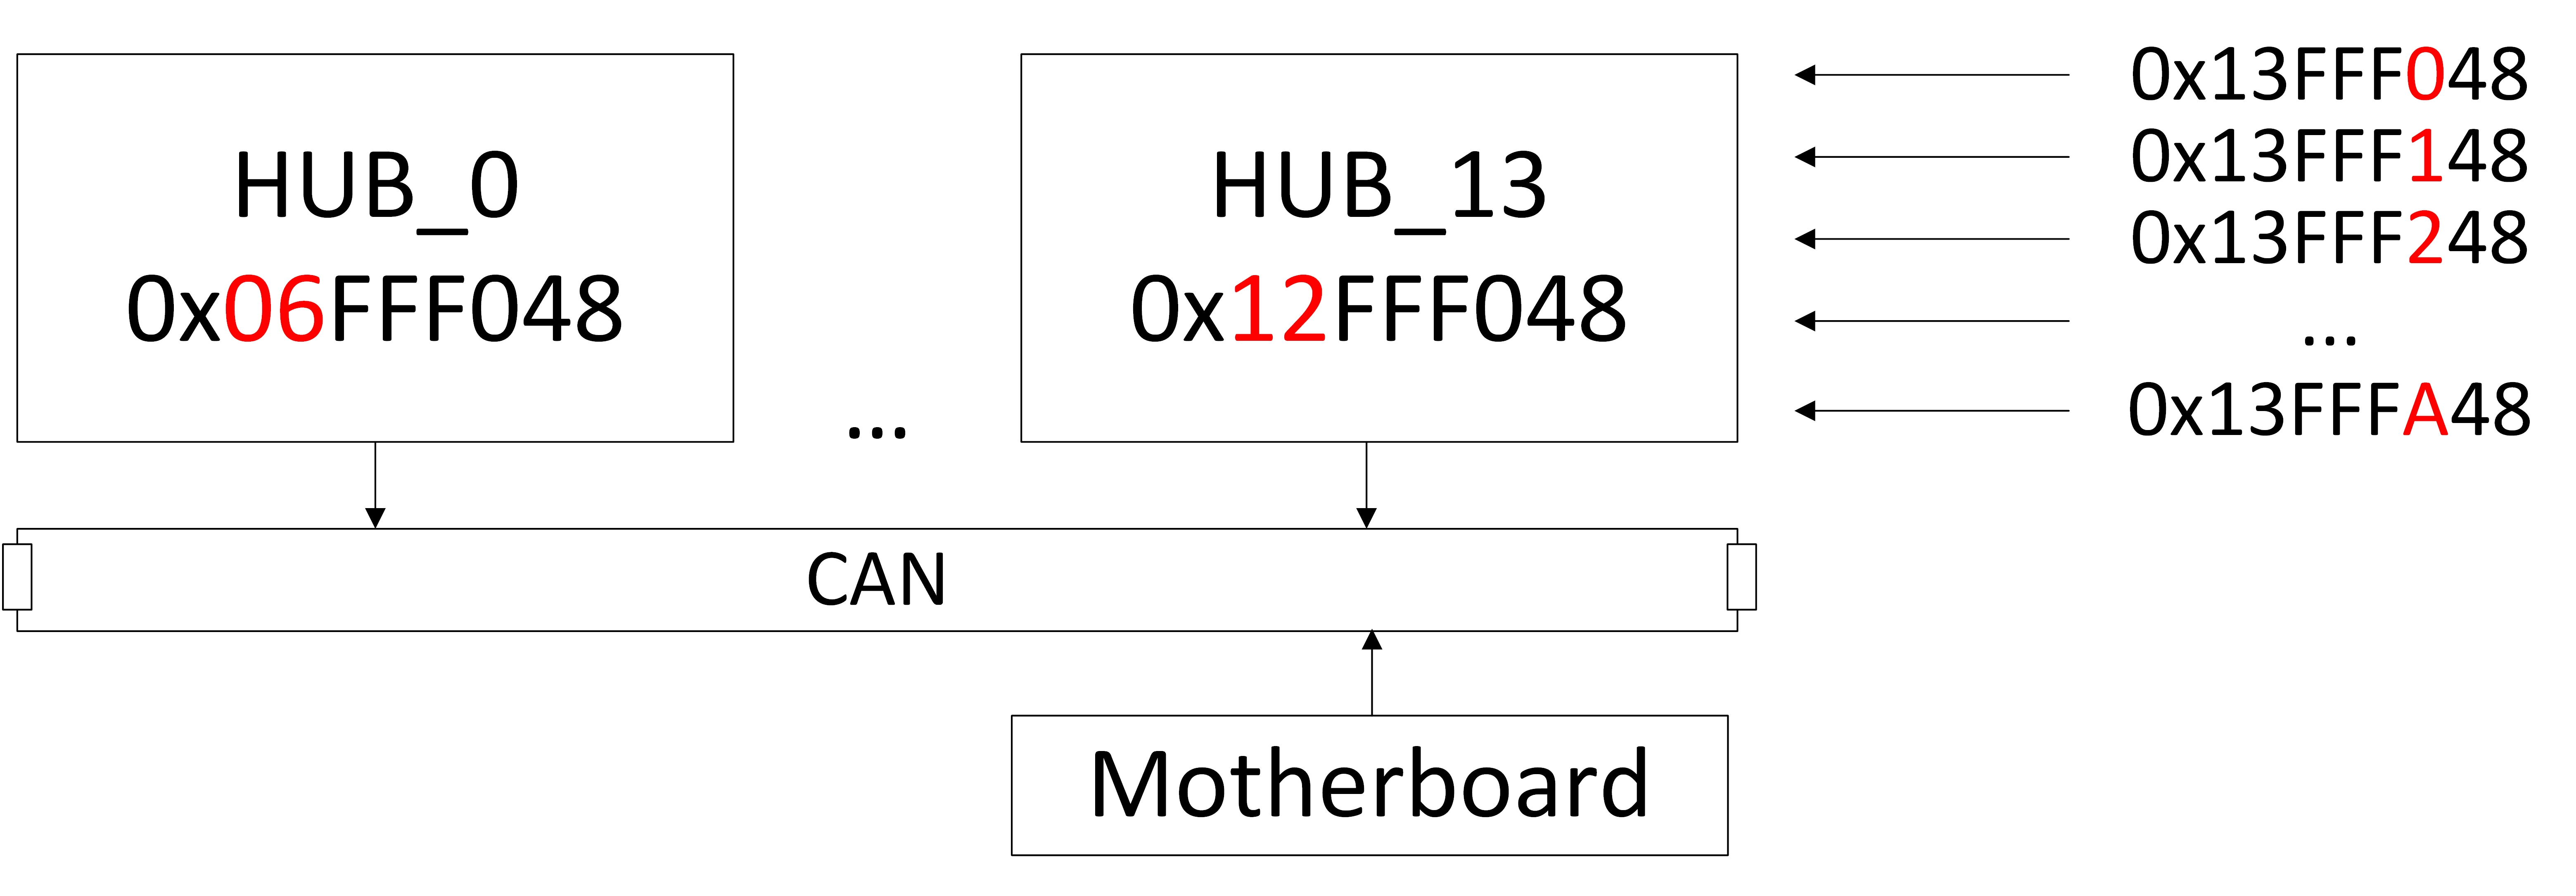
\includegraphics[width=0.75\textwidth]{figures/Adresowanie.JPG}
\caption{Kodowanie adres�w w ramce $CAN$}
\label{fig:adresowanie}
\end {figure}

\subsubsection{Filtry akceptacyjne} \label{ssec:filtry}
Kontroler magistrali $CAN$ wyposa�ony jest w w sprz�towe filtry akceptacyjne. Na ka�dy z dw�ch interfejs�w $CAN$ przypada 14 filtr�w akceptacyjnych. Bank filtr�w mo�na skonfigurowa� na kilka sposob�w. Po pierwsze nale�y wybra� wersj� wspieranego protoko�u (wi�cej o wersjach protoko�u $CAN$ w \hyperref[sec:can]{Sekcji~\ref*{sec:can}: G��wna magistrala komunikacyjna}). W przypadku omawianego systemu jest to wersja z rozszerzonym polem identyfikatora. Programista uzyskuje dost�p do 32-bitowych rejestr�w, kt�re mo�na ustawi� w tryb listy identyfikator�w lub maskowania. Filtrowanie na podstawie listy identyfikator�w polega na por�wnaniu identyfikatora nadchodz�cej wiadomo�ci z identyfikatorem znajduj�cym si� w 32-bitowym rejestrze. Tryb maskowania polega na dodatkowym zdefiniowaniu maski, kt�ra wskazuje, kt�re bity identyfikatora nadchodz�cej wiadomo�ci maj� zosta� por�wnane z rejestrem w pami�ci procesora. Nale�y pami�ta� o tym, �e identyfikatory posiadaj� tylko 29 bit�w, a warto�� w rejestrze jest wyr�wnana do lewej, czyli w stron� najbardziej znacz�cego bitu. Odwo�uj�c si� do warto�ci w rejestrze nale�y przesun�� go o 3 bity w lewo, aby odczytywa� 29 najbardziej znacz�cych bit�w. Przyk�ad mo�liwego zastosowania filtru maskuj�cego przedstawiono na \hyperref[listing:mask]{Listingu~\ref*{listing:mask}}.

\noindent \begin{minipage}{\textwidth}
\begin{lstlisting}[captionpos=b, belowcaptionskip=8pt, caption=Maska akceptacyjna $CAN$, label=listing:mask]
#define CAN_ID_HUB6 0x0CFFF048 // 0 1100 1111 1111 1111 0000 0100 1000
#define CAN_ID_MASK 0x1F000000 // 1 1111 0000 0000 0000 0000 0000 0000
CAN_FilterInitStructure.CAN_FilterIdHigh=(uint16_t)((CAN_ID_HUB6<<3)>>16);
CAN_FilterInitStructure.CAN_FilterIdLow=(uint16_t)(CAN_ID_HUB6<<3);
CAN_FilterInitStructure.CAN_FilterMaskIdHigh=(uint16_t)((CAN_ID_MASK<<3)>>16);
CAN_FilterInitStructure.CAN_FilterMaskIdLow=(uint16_t)(CAN_ID_MASK<<3);
\end{lstlisting}
\end{minipage}

W systemie wykorzystano tryb maskowania filtr�w. Utworzono bank 13 filtr�w przypisanych do interfejsu $CAN1$. Ka�dy filtr ma t� sam� mask� 0x1F000000, przedstawion� na \hyperref[listing:mask]{Listingu~\ref*{listing:mask}} oraz w�asne ID, na kt�re maska jest nak�adana. Por�wnywanych jest tylko 5 pierwszych bit�w (zamiast 29) identyfikatora, co skraca czas odbierania wiadomo�ci. Proces akceptacji wiadomo�ci (\hyperref[fig:accept]{Rysunek~\ref*{fig:accept}}) polega na wykonaniu iloczynu logicznego maski oraz identyfikatora nadchodz�cej wiadomo�ci, a nast�pnie por�wnaniu maskowanych bit�w (gdzie maska przyjmuje warto�� 1) z identyfikatorem zapisanym w rejestrze procesora. W przypadku niezgodno�ci operacja powtarzana jest dla kolejnych filtr�w. Przy dalszej niezgodno�ci, wiadomo�� jest ignorowana (bez u�ycia zasob�w procesora). W przypadku udanego por�wnania, wiadomo�� trafia do skrzynki odbiorczej i wywo�ywane jest przerwanie odbioru wiadomo�ci. Dzi�ki formie maski por�wnaniu ulega tylko segment A identyfikatora (patrz: \hyperref[fig:identyfikatory]{Rysunek~\ref*{fig:identyfikatory}}).

\begin  {figure} [h] 
\centering
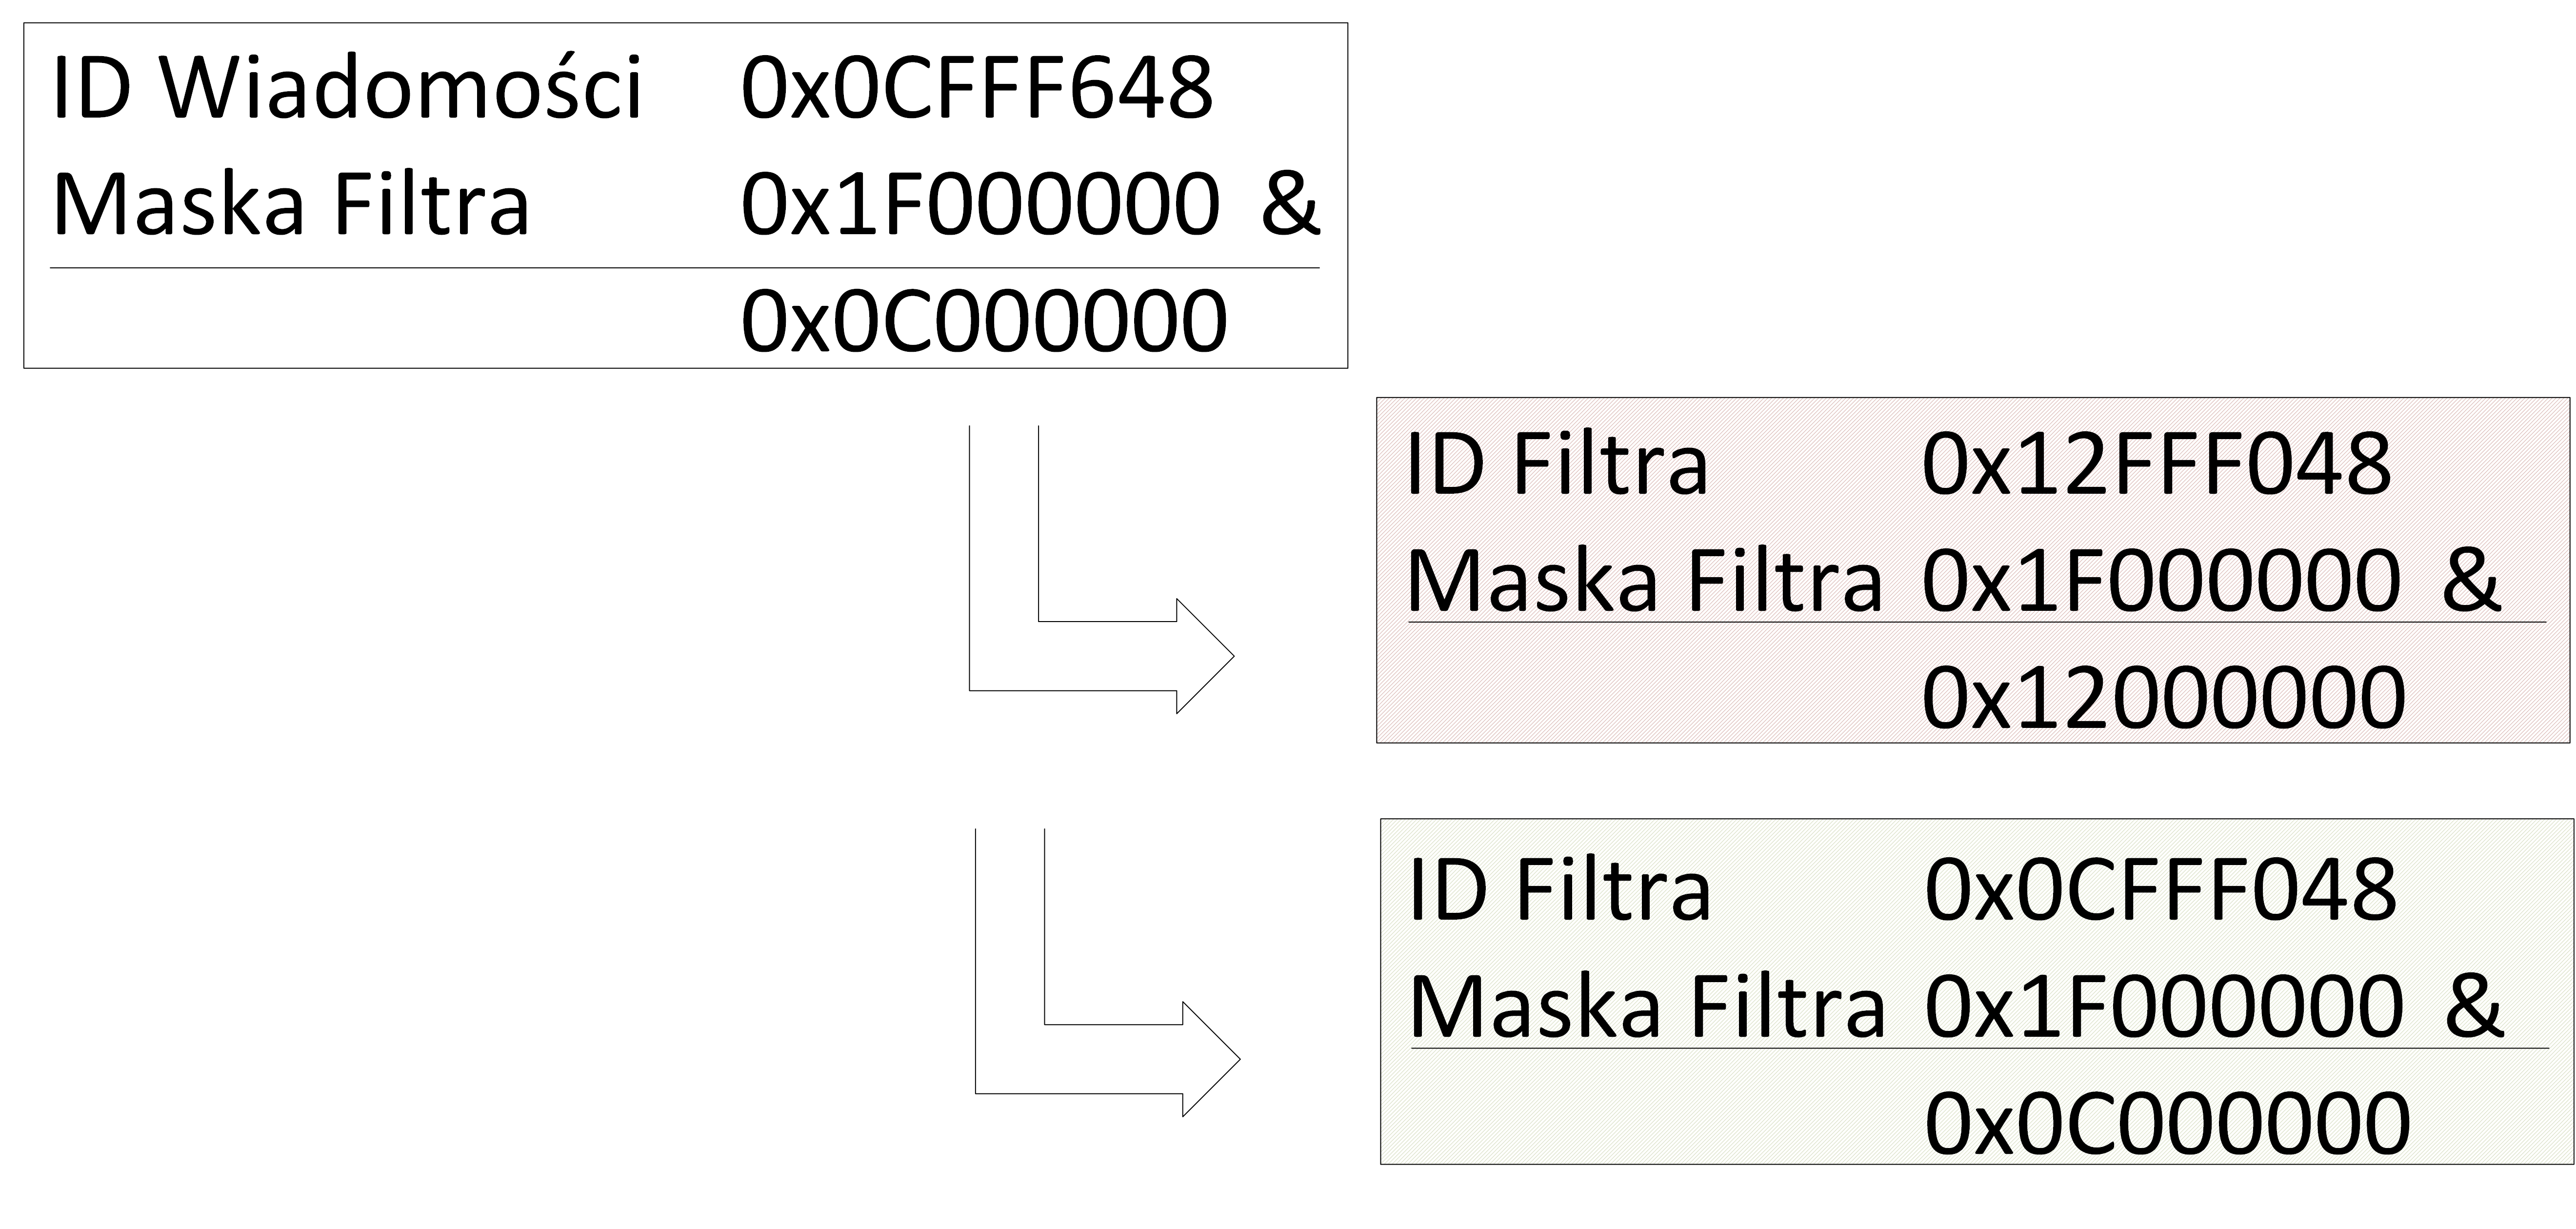
\includegraphics[width=0.75\textwidth]{figures/accept.JPG}
\caption{Filtrowanie wiadomo�ci $CAN$}
\label{fig:accept}
\end {figure}

Do skrzynki odbiorczej trafia wiadomo�� z numerem filtru, czyli po�rednio z numerem w�z�a, kt�ry wiadomo�� wys�a�. Numer filtru przechowywany jest wraz z wiadomo�ci� w zmiennej $FMI$ (Filter Match Index). Spos�b numeracji $FMI$ przedstawiono w \hyperref[ch:eksperyment]{Rozdziale~\ref*{ch:eksperyment}: Badania eksperymentalne}. Program ma za zadanie por�wnanie tylko jednego bajtu identyfikatora (segmentu B) w celu odkrycia, kt�ry kana� przetwornika ADC zosta� zapisany do pola danych wiadomo�ci lub kt�r� informacj� wys�a� sterownik silnika. Por�wnanie dokonywane jest dopiero na poziomie interfejsu u�ytkownika.\\
\\
Niezale�nie od tego czy chce si� u�ywa� filtr�w akceptacyjnych czy nie, trzeba zdefiniowa� chocia� jeden filtr. W przeciwnym wypadku �adna wiadomo�� nie zostanie przyj�ta do programu.

\subsubsection{Transceiver CAN}
Kontroler magistrali $CAN$, w kt�ry wyposa�ony jest procesor, posiada dwie asynchroniczne linie danych. S� to jednokierunkowe linie $Rx$ oraz $Tx$. Aby pod��czy� kontroler do magistrali, na kt�rej wyst�puj� sygna�y $CAN$ $High$ oraz $CAN$ $Low$, nale�y szeregowe komunikaty binarne skonwertowa� na sygna� r�nicowy. Konwersj� komunikatu oraz dostosowaniem napi�� zajmuje si� Transceiver $CAN$. Modu� u�yty w projekcie to L9616~\cite{manual:can}. Aby uchroni� uk�ad g��wnego komputera od szpilek wysokich napi��, kt�re mog�yby przedosta� si� z magistrali, oraz od zak��ce� na masie, u�yto dwukana�owej izolacji galwanicznej w module ISO7221~\cite{manual:iso}. Izoluje ona zar�wno linie sygna�owe, jak i zasilania, oddzielaj�c uk�ad Transceivera od g��wnego komputera. Schemat przedstawiono na \hyperref[fig:transceiver]{Rysunku~\ref*{fig:transceiver}}.

\begin  {figure} [h] 
\centering
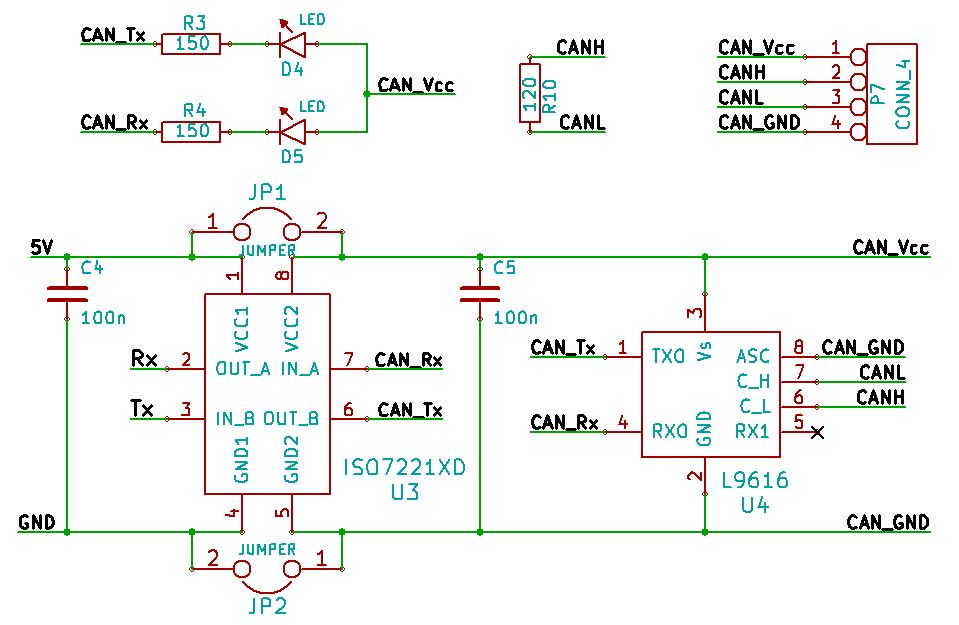
\includegraphics[width=0.75\textwidth]{figures/Transceiver_schemat.JPG}
\caption{Schemat Tranceivera $CAN$ z izolacj� galwaniczn�}
\label{fig:transceiver}
\end {figure}

Zworki JP1 oraz JP2 umo�liwiaj� zasilenie magistrali z tego samego �r�d�a, z kt�rego zasilany jest g��wny komputer pok�adowy (lub HUB, gdy� w obu urz�dzeniach wyst�puj� bli�niacze uk�ady Transceiver�w). Mo�na r�wnie� w ten spos�b zasili� urz�dzenia pod��czone do magistrali. Diody sygnalizuj�, czy aktualnie odbywa si� transmisja. 

\subsubsection{Pr�dko�� transmisji}
Standard SAE J1939 wymusza ustawienie w systemie pr�dko�ci przesy�u danych r�wnej 250~kb/s. Komunikacja jest asynchroniczna, wi�c wszystkie w�z�y musz� mie� zaimplementowany w�asny system zegarowy, kontroluj�cy pr�dko�� wysy�ania wiadomo�ci. Komputer pok�adowy taktowany jest sygna�em o cz�stotliwo�ci 168~MHz, potrzebne jest wyliczenie odpowiedniego preskalera, kt�ry zapewni ��dan� cz�stotliwo��. Aby u�y� \hyperref[eq:tq]{Wzoru~\ref*{eq:tq}} nale�y pami�ta�, �e kontroler magistrali taktowany jest przez wewn�trzny preskaler magistrali APB1 r�wny 4. St�d cz�stotliwo�� taktuj�ca kontroler magistrali jest r�wna 42~MHz. Mo�na teraz wyprowadzi� wz�r na d�ugo�� trwania bitu ze \hyperref[eq:baud]{Wzoru~\ref*{eq:baud}}:

\begin{equation}
T=\frac{1}{BaudRate}=1/250kb=4 \cdot 10^{-6}=4\mu s
\end{equation}

4 $\mu$s s� wielokrotno�ci� kwantu czasu. Ilo�� kwant�w czasu musi si� zawiera� pomi�dzy 8 a 25. W systemie podzielono bit na 8 cz�ci, uzyskuj�c d�ugo�� kwantu r�wn� 500~ns. Na podstawie tej decyzji oraz \hyperref[eq:tq]{Wzoru~\ref*{eq:tq}} dobrano preskaler r�wny:

\begin{equation}
BRP=t_{q} \cdot f_{clk} = 5 \cdot 10^{-7} \cdot 42 \cdot10^{6} = 21
\end{equation}

Nast�pnym etapem jest dob�r d�ugo�ci trwania segment�w $BS1$ oraz $BS2$. Przyj�to, �e punkt pr�bkowania powinien przypada� w okolicy 87,5\% czasu trwania bitu. Warto�� ta pochodzi z for�w internetowych i jest powszechnie stosowana w sieciach $CAN$ (m.in. w protokole $CANopen$). Istnieje jednak du�a grupa os�b, kt�ra uwa�a takie podej�cie za b��dne, umieszczaj�c punkt pr�bkowania w 30\% lub 95\%. Aby dobra� d�ugo�ci trwania segment�w wyprowadzono zale�no�� na podstawie \hyperref[eq:baud]{Wzoru~\ref*{eq:baud}}:

\begin{equation}
\frac{t_{BS1}+t_{q}}{t_{q}+t_{BS1}+t_{BS2}}=87,5\%
\end{equation}

W mianowniku wyra�ono ca�kowity czas trwania bitu, kt�ry r�wny jest $8t_{q}$, st�d:

\begin{equation}
t_{BS1}=(8 \cdot 87,5\%-1)t_{q}=6t_{q}
\end{equation}
\begin{equation}
t_{BS2}=t_{q}
\end{equation}
Komunikacja przebiega pomy�lnie w �rodowisku wolnym od zak��ce� przy ma�ym nat�eniu ruchu na sieci. Dob�r czas�w b�dzie musia� zosta� zweryfikowany w rzeczywistym systemie w rzeczywistych warunkach po pod��czeniu wszystkich w�z��w, okablowania oraz rozmieszczenia element�w wewn�trz pojazdu. Wtedy segment propagacji sygna�u b�dzie musia� zosta� dobrany metod� eksperymentaln�.

\subsection{Obs�uga karty SD}
Obs�uga karty SD odbywa si� poprzez protok� $SD$ $Bus$, przy u�yciu zintegrowanego peryferium $SDIO$ (Secure Digital Input Output) mikrokontrolera. $SDIO$ s�u�y do obs�ugi funkcji wej�cia/wyj�cia urz�dze� zgodnych ze standardem SD~\cite{spec:sd}. Wyr�niane s� trzy fizyczne topologie sieci. Przy u�yciu fizycznej warstwy protoko�u $SPI$, $SD$ $Bus$ z jedn� lub czterema liniami danych. W projekcie u�yto standardu 4-bitowego. Na \hyperref[fig:sd_schemat]{Rysunku~\ref*{fig:sd_schemat}} pokazano realizacj� warstwy fizycznej protoko�u $SD$ $Bus$ u�yt� w projekcie. Linie danych i komend musz� posiada� podci�gni�cia do zasilania. Interfejs $SPI$ oraz $SD$ $Bus$ 1-bitowy (na kt�rym wykonywano testy) nie s� kompatybilnymi interfejsami. Nale�y przygotowa� odpowiednio warstw� fizyczn� aby unikn�� problem�w podczas implementacji programu.

\begin  {figure} [h] 
\centering
\includegraphics[width=0.5\textwidth]{figures/sd_schemat.JPG}
\caption{Schemat pod��czenia slotu karty SD zgodnie z $SD$ $Bus$ 4-bitowym}
\label{fig:sd_schemat}
\end {figure}

Wszystkie karty SD s� kompatybilne ze standardem $SDIO$, kt�ry zapewnia pe�n� obs�ug� w ich ograniczonym zakresie (bez u�ycia polece� wej�cia/wyj�cia). Do urz�dze� wykorzystuj�cych pe�ni� potencja�u protoko�u $SDIO$ zalicza si� mi�dzy innymi kamery, karty bluetooth i odbiorniki GPS. Obs�uga tych urz�dze� r�ni si�, ale wszystkie s� zgodne ze standardem $SDIO$~\cite{spec:sdio}.\\
Bazuj�c na za�o�eniach projektu zaimplementowano obs�ug� karty SD przez kontroler $DMA$, skracaj�c czas operacji na plikach. U�yta w tym celu biblioteka jest autorstwa Tilen'a Majerle~\cite{lib:sd}. Tilen Majerle zapewnia sta�e wsparcie dla biblioteki i udziela odpowiedzi na pytania u�ytkownik�w. U�atwia to w znacz�cym stopniu implementacj� biblioteki i jej p�niejsze u�ycie oraz zintegrowanie z pozosta�� cz�ci� programu. 

\subsubsection{Zapis do pliku}
Wa�nym elementem biblioteki jest funkcja pozwalaj�ca na zapisywanie sformatowanego tekstu do pliku \textit{fprintf (FILE * stream, const char * format, ... )}. Przyk�ad u�ycia  funkcji przedstawiono na \hyperref[listing:fprintf]{Listingu~\ref*{listing:fprintf}}. Nale�y okre�li� plik docelowy, oraz ramk� $CAN$, kt�r� chce si� zapisa� do pliku. Format danych w pliku, kt�re s� ju� wst�pnie posortowane na jednostki pomiarowe, to zapis w formacie kodu ASCII szesnastkowej postaci identyfikatora, kodu DLC oraz danych. Z identyfikatora mo�na odczyta�, kt�rego wej�cia przetwornika ADC dotyczy ramka lub w przypadku HUB\_6, kt�ry zestaw parametr�w przesy�any jest przez sterownik silnika. Dzi�ki kodowi DLC wiadomo ile nast�pi po nim bajt�w danych. Zapis ko�czy si� znakiem nowej linii '$\backslash$n'. Na \hyperref[fig:zapis]{Rysunku~\ref*{fig:zapis}}.

\begin  {figure} [h] 
\centering
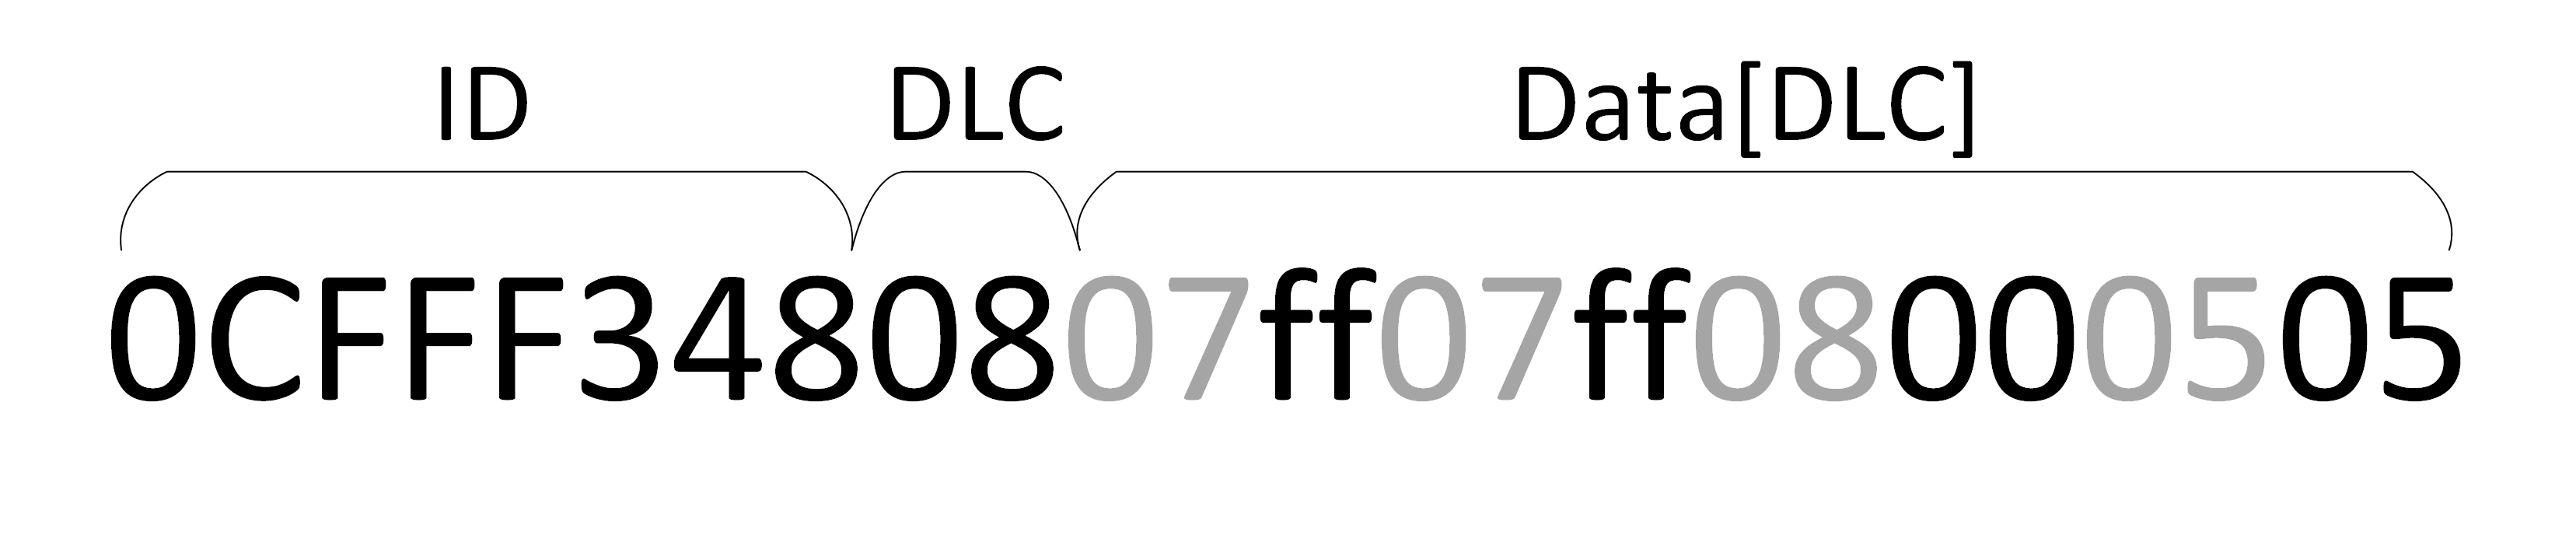
\includegraphics[width=0.75\textwidth]{figures/zapis.JPG}
\caption{Przyk�ad ramki zapisanej w pliku HUB\_6.txt}
\label{fig:zapis}
\end {figure}

\noindent\begin{minipage}{\textwidth}
\begin{lstlisting}[captionpos=b, belowcaptionskip=8pt, caption=Funkcja zapisu danych na kart� SD, label=listing:fprintf]
void f_SendCanFrame (FIL* file, uint8_t sieze, CanRxMsg RxMessage)
{
	uint8_t i =0;
	f_printf(&file[RxMessage.FMI],"%08x%02x",RxMessage.ExtId,RxMessage.DLC);
	for(;i<RxMessage.DLC;i++)
	{
		f_printf(&file[RxMessage.FMI],"%02x",RxMessage.Data[i]);
	}
	f_printf(&file[RxMessage.FMI],"\n");
}
\end{lstlisting}
\end{minipage}

Podczas inicjalizacji systemu otwieranych jest 13 plik�w, kt�re przechowuj� informacje o poszczeg�lnych jednostkach pomiarowych. Numer pliku, do kt�rego maj� trafi� zapisane dane, definiuje filtr, kt�ry dopu�ci� dane do systemu, czyli zmienna $FMI$ struktury typu $CanRxMsg$. Pliki s� zamykane przed wyj�ciem karty ze slotu SD oraz podczas wykrycia opadaj�cego zbocza sygnalizuj�cego od��czenie napi�cia zasilania przez jeden z g��wnych wy��cznik�w w poje�dzie. Realizacja polega na obs�udze przerwa� zewn�trznych, w kt�rych wywo�ywane s� funkcje fopen (przy w�o�eniu karty SD do slotu lub w��czeniu napi�cia zasilaj�cego - \hyperref[listing:fopen]{Listing~\ref*{listing:fopen}}) oraz fclose (przy wyj�ciu karty SD ze slotu lub zaniku napi�cia zasilaj�cego - \hyperref[listing:fclose]{Listingu~\ref*{listing:fclose}}).\\

\noindent\begin{minipage}{\textwidth}
\begin{lstlisting}[captionpos=b, belowcaptionskip=8pt, caption=Funkcja otwarcia wielu plik�w, label=listing:fopen]
FRESULT f_open_files(FIL* file, uint8_t size)
{
	FRESULT res;
	char bufor[10];	
	int i=0;
	for (;i<size;i++)
	{
		sprintf(bufor,"HUB_%u.txt",i);
		res = f_open(&file[i], bufor, FA_OPEN_ALWAYS | FA_WRITE);
		if (res != FR_OK)
		{
			return res;
		}
		res = f_lseek(&file[i], f_size(&file[i])); // append file
		if (res != FR_OK)
		{
			return res;
		}
	}
	return res;
}
\end{lstlisting}
\end{minipage}

\noindent\begin{minipage}{\textwidth}
\begin{lstlisting}[captionpos=b, belowcaptionskip=8pt, caption=Funkcja zamkni�cia wielu plik�w, label=listing:fclose]
FRESULT f_close_files(FIL* file, uint8_t size)
{
	FRESULT res;
	int i=0;
	for (;i<size;i++)
	{
		res = f_close(&file[i]);
		if (res != FR_OK)
		{
			return res;
		}
	}
	return res;
}
\end{lstlisting}
\end{minipage}

Mikrokontroler posiada dwa kontrolery $DMA$, ka�dy maj�cy 8 strumieni dziel�cych si� na 8 kana��w. Utworzona w ten spos�b macierz 64 p�l oraz przypisane do nich peryferia przedstawiono w tabelach 35. oraz 36. RM0090 Reference manual~\cite{manual:stm32f4}. R�nice w obs�udze karty przy u�yciu protoko�u $SPI$, $SD$ $Bus$ oraz badania czasu zapisu zawarto w \hyperref[ch:eksperyment]{Rozdziale~\ref*{ch:eksperyment}: Badania eksperymentalne}.\\
Polecenia u�yte podczas obs�ugi karty SD s� standardowymi zestawami komend oraz argument�w, wysy�anych odpowiednio po liniach danych i komend. Przyk�adowe komendy om�wione s� w specyfikacji Secure Digital Card Product Manual (Sekcja 4.7 Commands)~\cite{manual:sandisk}. 

\subsection{Obs�uga modu�u XBee}
Wyr�niane s� dwie wersje modu�u XBee. Jedna zawiera wbudowan� anten� radiow�, a druga umo�liwia wyprowadzenie anteny poza p�ytk� PCB. Zdecydowano si� na wariant urz�dzenia z zewn�trzn� anten� w celu zwi�kszenia zasi�gu.  Zrezygnowano z pin�w $RTS$ oraz $CTS$, rezygnuj�c tym samym z kontroli przep�ywu danych, ale przy dobrze zaprogramowanej komunikacji nie s� one wymagane. Modu� dzia�a jednokierunkowo, bez sprawdzania, czy wiadomo�� dotar�a do celu. Aby uzyska� szybszy przekaz danych ustawiono modu� w tryb transparentny (wi�cej w \hyperref[sec:sub:tryby]{Sekcji~\ref*{sec:sub:tryby}: Tryby pracy modu�u XBee}). Schemat modu�u przedstawiono na \hyperref[fig:xbee_schemat]{Rysunku~\ref*{fig:xbee_schemat}}.

\begin  {figure} [h] 
\centering
\includegraphics[width=0.5\textwidth]{figures/xbee_schemat.JPG}
\caption{Schemat pod��czenia radiowego modu�u XBee}
\label{fig:xbee_schemat}
\end {figure}

Komunikacja z modu�em odbywa si� dzi�ki zintegrowanemu w mikrokontrolerze modu�owi $UART$. Na linii $DOUT$ modu�u mikrokontrolera wysy�ana jest kopia ramki $CAN$, tak aby umo�liwi� jej podgl�d w interfejsie u�ytkownika. Jest to na�o�enie protoko�u $CAN$ na asynchroniczn� szeregow� pojedyncz� lini� danych. Ramka przesy�ana jest jako strumie�, czyli ci�g znak�w ASCII (tablica znak�w ko�cz�ca si� znakiem $NULL$). Jest to reprezentacja warto�ci ramki w systemie szesnastkowym. Do przes�ania sformatowanego tekstu po $UART$ u�yto funkcji \textit{USART\_SendCanFrame}, przedstawionej na \hyperref[listing:usart]{Listingu~\ref*{listing:usart}}.\\

\noindent\begin{minipage}{\textwidth}
\begin{lstlisting}[captionpos=b, belowcaptionskip=8pt, caption=Funkcja enkaspulacji danych na $UART$, label=listing:usart]
void USART_SendCanFrame (CanRxMsg RxMessage)
{
	int i = 0;
	char string[27];
	string[0]='\0';
	char b[9];
	b[0] = '\0';
	sprintf(b,"%08x",(unsigned int)RxMessage.ExtId);
	strcat(string,b);
	sprintf(b,"%02x",(unsigned int)RxMessage.DLC);
	strcat(string,b);
	for (;i<RxMessage.DLC;i++)
	{
		sprintf(b,"%02x",(unsigned int)RxMessage.Data[i]);
		strcat(string,b);
	}
	USART_printf("%s",string);
}
\end{lstlisting}
\end{minipage}
\\
Dla przyk�adu, chc�c przes�a� warto�� 0x01ABC, zostanie przes�ane s�owo "01abc", czyli ci�g znak�w 0x30 0x31 0x61 0x62 0x63 0x00. Takie podej�cie umo�liwia kontrol� ko�ca ramki $CAN$ (znak $NULL$). Ramka sk�ada si� tylko z identyfikatora $CAN$, kodu $DLC$ oraz p�l danych. D�ugo�� informacji w bajtach to:
\begin{equation}
ExtID+DLC+Data=4+1+DLC*1
\end{equation}
Maksymalna ilo�� danych to 8 bajt�w ($DLC = 8$), st�d maksymalna d�ugo�� komunikatu wynosi 13 bajt�w. W zapisie hexadecymalnym jest to 26 znak�w, kt�re stanowi� maksymaln� d�ugo�� ramki.\\

Aby rozpocz�� prac� z modu�em z w�asnymi ustawieniami transmisji nale�y ustawi� pr�dko�� transmisji ($BD$), parzysto�� ($NB$) i bity stopu ($SB$). Wszystkie parametry modu�u mo�na zmienia� przy u�yciu komend AT (dost�pnych w Rozdziale 10. XBee�/XBee-PRO� ZB SMT RF Modules Datasheet~\cite{manual:xbee}). Aby u�ywa� komend nale�y wprowadzi� modu� w tryb odbioru komend AT przy u�yciu specjalnej komendy oraz parametr�w domy�lnych transmisji, czyli 9600 b/s, 1 bit stopu i brak bitu parzysto�ci.\\

Po zako�czeniu inicjalizacji mo�na albo poczeka�, a� modu� sam wr�ci do trybu wysy�ania danych przez anten�, albo wymusi� powr�t. Po powrocie w tryb przesy�ania danych, modu� powraca do buforowania danych z magistrali szeregowej. Dioda sygnalizuje, czy urz�dzenie zosta�o sparowane z odbiornikiem czy nie, zmieniaj�c cz�stotliwo�� �wiecenia.

\subsection{Zasilanie}
P�ytka ewaluacyjna STM32F4-Discovery do poprawnego dzia�ania wszystkich peryferi�w wymaga napi�cia 5 V. Zdecydowano, �e napi�cie to b�dzie dostarczane przez przetwornice step-down firmy POLOLU o pr�dzie wyj�ciowym 600 mA. Na wej�ciu przetwornicy zastosowano diod� prostownicz� jako zabezpieczenie przed pod��czeniem odwrotnej polaryzacji napi�cia oraz bezpiecznik polimerowy. Na wej�ciu oraz wyj�ciu przetwornicy zosta�y umieszczone kondensatory tantalowe o warto�ciach 47 uF w celu filtrowania napi�cia zasilania.

\subsection{System przerwa�}
Przy obs�udze tak wielu uk�ad�w peryferyjnych wa�ne jest zachowanie pewnego systemu priorytet�w przerwa�, kt�re mog� zosta� zg�oszone jednocze�nie. S�u�y do tego uk�ad $NVIC$ (Nested Vector Interrupt Controller) zintegrowany w procesorze. W systemie wyr�niamy nast�puj�ce przerwania:
\begin{itemize}
\item odbioru wiadomo�ci na magistrali $CAN$,
\item ko�ca przesy�u wiadomo�ci przez kontroler $DMA$,
\item ko�ca przetwarzania wiadomo�ci przez $SDIO$,
\item wsuni�cia/wysuni�cia karty SD do/ze slotu,
\item pojawienia si� lub zanikni�cia napi�cia zasilaj�cego,
\item od timera watchdog,
\item od timer�w pomocniczych.
\end{itemize}

Procesor umo�liwia zdefiniowanie grup przerwa�, kt�re maj� wy�szy priorytet. W systemie u�yto dw�ch grup g��wnych (preemption priority group) z siedmioma podgrupami (sub priority group) w celu uszeregowania priorytet�w. Zapewniono najwy�szy priorytet przerwaniu zaniku zasilania oraz wysuni�ciu karty SD, aby nie utraci� zebranych na karcie danych. Kolejnym przerwaniem jest timer watchdog. W przypadku, gdy podczas obs�ugi dowolnego przerwania (lub wykonywania p�tli $while()$), system zawiesi si� i nie zostanie obs�u�one przerwanie od timera watchdog, system ulegnie resetowi. Kolejn� grup� s� przerwania odpowiedzialne za timery, nast�pnie za odbi�r ramki $CAN$. Taki system priorytet�w zapewnia spe�nienie czasowych ogranicze� narzuconych systemowi przez ilo�� operacji do wykonania w okresie pr�bkowania przetwornik�w. Spe�nienie wymog�w czasowych przeanalizowano w  \hyperref[ch:eksperyment]{Rozdziale~\ref*{ch:eksperyment}: Badania eksperymentalne}.\\

\section{Rozproszone jednostki pomiarowe}
\textit{Autor: Jakub Baranowski}\\ \\

%G��wne zadanie Rozproszonej Jednostki Pomiarowej ($HUB$) to dokonywanie pomiaru wielko�ci fizycznych mierzonych przez czujniki rozmieszczone w bolidzie. Za standard analogowego sygna�u wej�ciowego przyj�to 0-12 V. \newline

Uk�ad Jednostki Pomiarowej sk�ada si� z 3 odseparowanych galwanicznie cz�ci: pomiarowej, mikrokontrolerowej i transmisji $CAN$.\newline

Uk�ad realizuj�cy dzia�anie Jednostki to STM32f103, zapewniaj�c peryferia pomiarowe jak i komunikacyjne.
\subsection{Mikrokontroler}

Mikrokontroler STM32f103 pochodzi z rodziny uk�ad�w o rdzeniu Cortex\texttrademark-M3. Dost�pny od paru lat na rynku, sprawdza si� w rozwi�zaniach wymagaj�cych ma�ego i prostego kontrolera. Szereg peryferi�w, w kt�re wyposa�ony jest ten uk�ad, stawia go w kategorii uniwersalno�ci nie osi�galnej przez inne uk�ady na rynku tej klasy. Najwa�niejsze peryferia wykorzystane w Hubie to:\newline
\begin{itemize}
	\item Dwa 12 bitowe przetworniki analogowo-cyfrowe, potrafi�ce obs�u�y� do 16 kana��w
	\item Interfejs komunikacyjny $CAN$ 2.0B
\end{itemize}

Uk�ad dostarcza tak�e 7 timer�w sprz�towych, kt�re mog� pracowa� w wielu zaawansowanych trybach. Do wykonywania pomiar�w z okre�lonym pr�bkowaniem wystarcz� podstawowe tryby dzia�ania dostarczonych timer�w.

\subsection{Separacja sygna��w analogowych}
Dokonywanie pomiaru odbywa si� za pomoc� kana��w $ADC$ mikrokontrolera. Przyj�ty standard napi�cia wymusza sprowadzenie poziom�w napi�� sygna�u do zakresu pracy przetwornika $ADC$. Podczas projektowania rozpatrywano 3 rozwi�zania:
\begin{itemize}
	\item Rezystancyjny dzielnik napi�cia
	\item Izolacja sygna��w analogowych przez zewn�trzny uk�ad $ADC$
	\item Izolacja sygna��w analogowych na uk�adzie IL300
\end{itemize}
Najprostszym rozwi�zaniem jest rezystancyjny dzielnik napi�cia. Jest to czw�rnik, kt�ry zapewnia uzyskanie okre�lonego stosunku pomi�dzy napi�ciem wej�ciowym, a wyj�ciowym~\cite{book:SE}. Rozwi�zanie tego typu w �aden spos�b nie zabezpiecza przed podaniem zbyt wysokiego napi�cia oraz wymusza aby sygna� analogowy by� mierzony wzgl�dem masy Jednostki Pomiarowej. \newline
\begin  {figure} [h] 
\centering
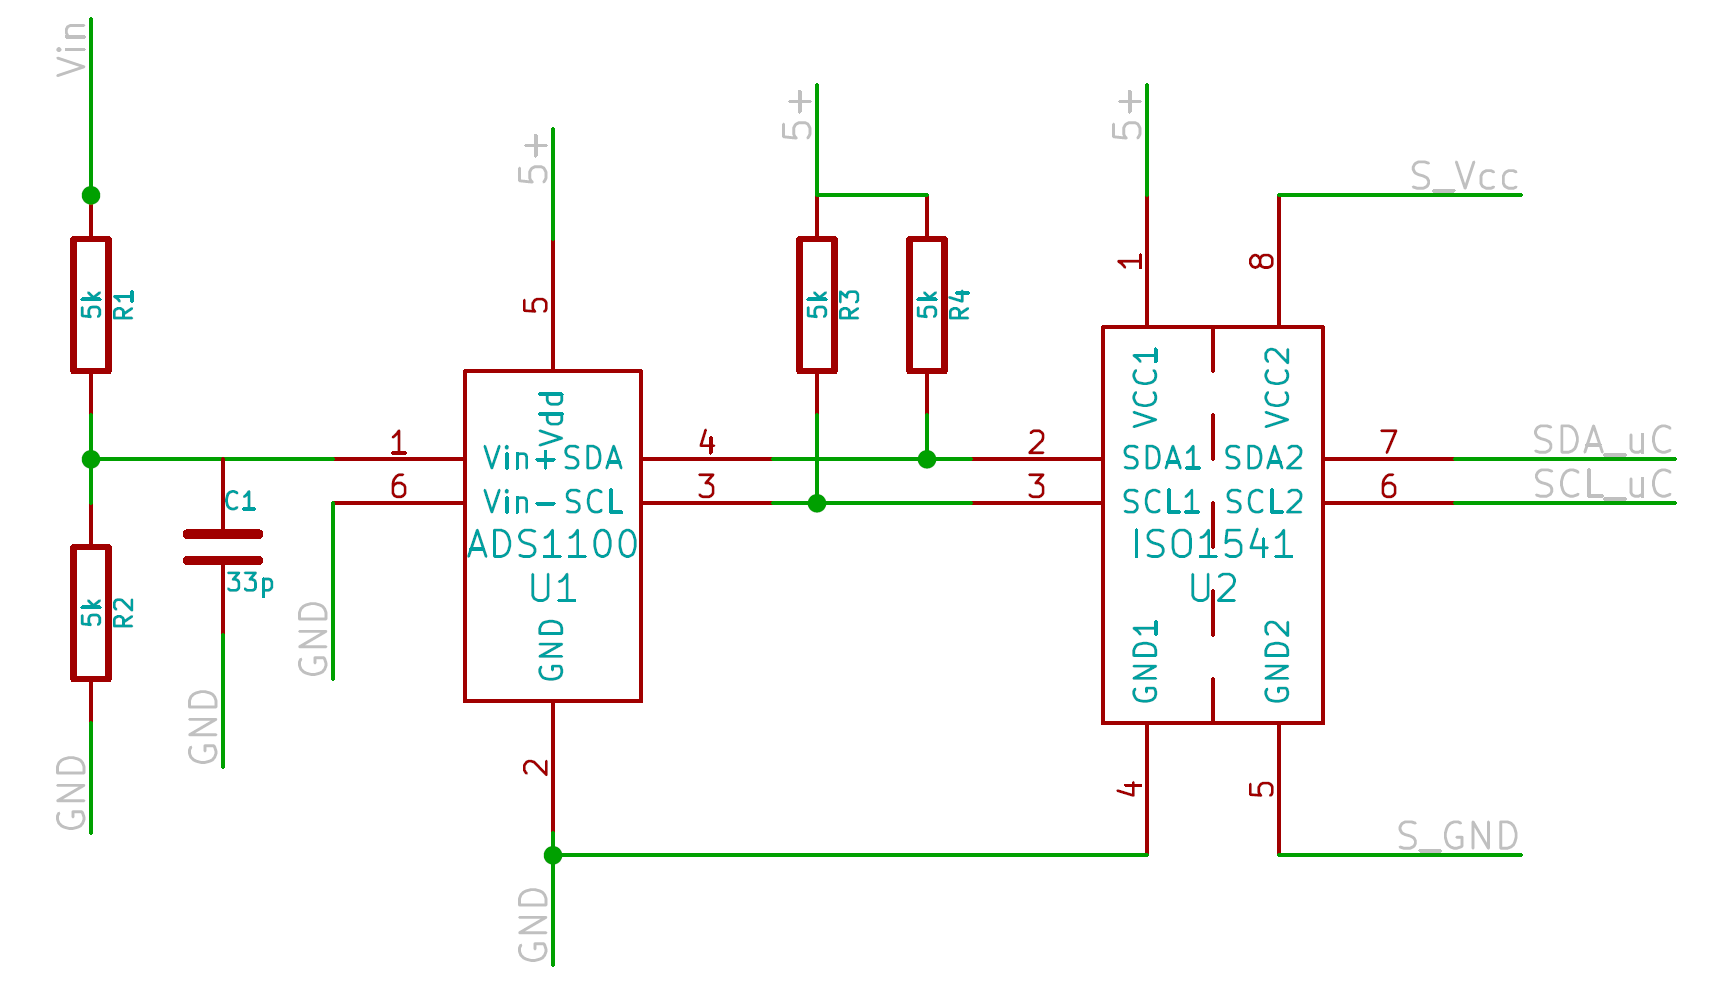
\includegraphics[width=0.75\textwidth]{figures/ADS1100.png}
\caption{Separacja analogowa przy u�yciu uk�adu ADS1100}
\label{fig:ADS}
\end {figure}

Nast�pn� metod� separacji, kt�r� brano pod uwag�, by�o wykorzystanie zewn�trznego uk�adu $ADC$, kt�ry przesy�a�by dane po odseparowanej magistrali danych. Zaprojektowane rozwi�zanie wida� na \hyperref[fig:ADS]{Rysunku~\ref*{fig:ADS}}. Zosta�o odrzucone, poniewa� przetwornik wymaga� zasilania o napi�ciu 5 V, co komplikowa�o uk�ad po stronie nieseparowanej. Dodatkowo takie rozwi�zania podwy�sza�o znacz�co koszt uk�adu. Rozwi�zanie to sprawdzi�o by si� w aplikacjach w kt�rych zale�y nam na wysokiej dok�adno�ci pomiar�w bez wprowadzania przek�ama�, kt�re pojawiaj� si� przy separacji analogowej.\newline

Ostatnia opcja, kt�ra zosta�a wybrana to separacja przy u�yciu uk�adu IL300. Uk�ad IL300 posiada jedn� diod� nadawcz� i dwie diody odbiorcze. Konfiguracja taka pozwala stworzy� po stronie pierwotnej, sprz�enie przez jedn� z diod odbiorczych, steruj�ce pr�dem diody nadawczej. Kompensuje to nieliniowo�� �wiecenia diody nadawczej wzgl�dem jej pr�du. Na stronie wt�rnej uk�adu IL300 mamy drug� diod� odbiorcz�, kt�rej pr�d jest zale�ny liniowo od pr�du diody odbiorczej po stronie pierwotnej~\cite{manual:DesIL300}.\newline

\begin  {figure} [h] 
\centering
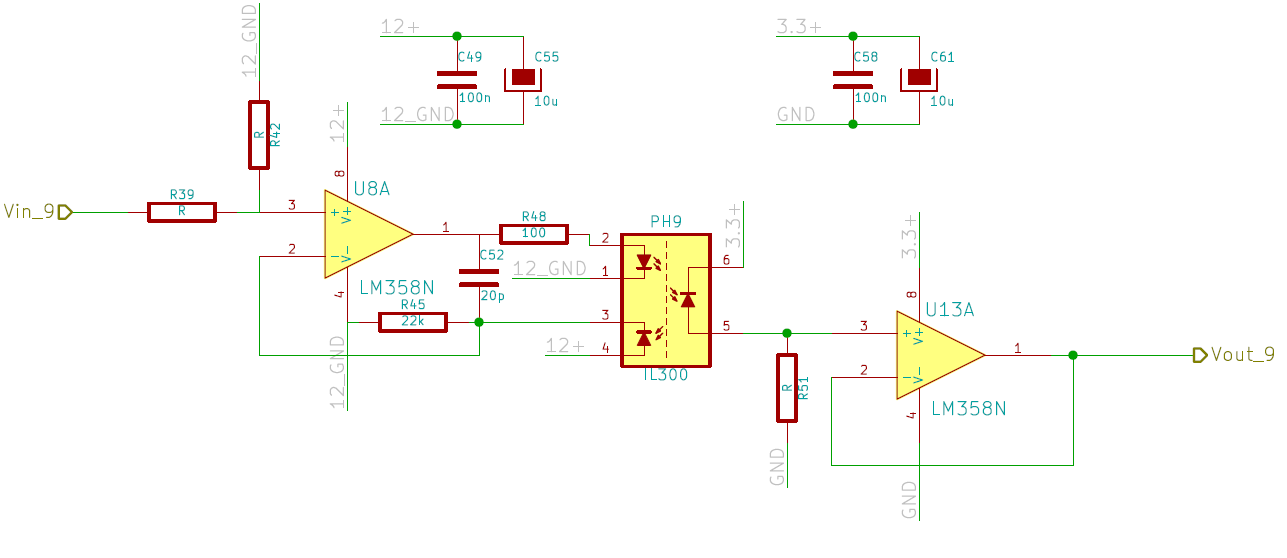
\includegraphics[width=0.75\textwidth]{figures/Il300.png}
\caption{Separacja analogowa przy u�yciu uk�adu IL300}
\label{fig:IL300}
\end {figure}

Na \hyperref[fig:IL300]{Rysunku~\ref*{fig:IL300}} zosta�a pokazana realizacja separacji na uk�adzie IL300. Po stronie pierwotnej mamy uk�ad $U8A$, kt�ry przez sprz�enie zwrotne linearyzuje diod� nadawcz�.  Na dodatnie wej�cie wzmacniacza wchodzi sygna� mierzony podzielony przez dzielnik napi�cia. Sygna� ten jest por�wnywany z napi�ciem na rezystorze, kt�re jest wymuszone przez pr�d p�yn�cy przez diod� odbiorcz�. Pr�d diody odbiorczej jest sterowany przez �wiecenie si� diody nadawczej, kt�ra jest sterowana przez pr�d wzmacniacza~\cite{manual:DesIL300}. Wz�r na obliczenie warto�ci rezystora to:\newline
\begin{equation} \label{K1} I_F=\frac{V_{in}}{K_1 \cdot R_1} \end{equation}
gdzie:\newline
$I_F$ - pr�d diody nadawczej\newline
$V_{in}$ - napi�cie na wej�ciu nieodwracaj�cym wzmacniacza\newline
$K_1$-wzmocnienie strony pierwotnej transoptora\newline
$R_1$-Rezystor bocznikowy\newline

Wzmacniacz $U13A$ po stronie wt�rnej jest w konfiguracji wt�rnika napi�ciowego. Na wej�cie nieodwracaj�ce jest podane napi�cie odk�adaj�ce si� na boczniku rezystancyjnym. Przez bocznik p�ynie pr�d diody odbiorczej strony wt�rnej~\cite{manual:DesIL300}. Wz�r na obliczenie warto�ci rezystora to:\newline
\begin{equation} \label{K2} I_F=\frac{V_{out}}{K_2 \cdot R_2} \end{equation}
gdzie:\newline
$I_F$ - pr�d diody nadawczej\newline
$V_{out}$ - napi�cie na wyj�ciu wzmacniacza\newline
$K_2$-wzmocnienie strony wt�rnej transoptora\newline
$R_2$-Rezystor bocznikowy

\noindent Z podstawienia wzoru \ref{K1} do wzoru \ref{K2} dostajemy wz�r:\newline
\begin{equation} \label{Pod} \frac{V_{out}}{V_{in}}=\frac{K_2 \cdot R_2}{K_1 \cdot R_1} \end{equation}
W dokumentacji podano wsp�czynnik $K_3$, kt�ry r�wna si�:\newline
\begin{equation} \label{K3} K_3=\frac{K_2}{K_1} \end{equation}
Z tej zale�no�ci wynika ostateczny wz�r na rezystancje bocznik�w:\newline
\begin{equation} \label{Ost} \frac{V_{out}}{V_{in}}=\frac{K_3 \cdot R_2}{R_1} \end{equation}

\subsection{Przep�yw danych}
Zadaniem Jednostki Pomiarowej jest wysy�anie zebranych informacji do g��wnego komputera pok�adowego. Nie musi ona odbiera� �adnych wiadomo�ci, st�d maska r�wna jest 0x1FFFFFFF. Jest to maska, kt�ra sprawia, �e ka�dy bit nadchodz�cego identyfikatora musi si� zgadza� z ustawionym identyfikatorem filtra, czyli z identyfikatorem samej jednostki. Oznacza to, �e jednostka odczytuje tylko w�asne komunikaty. System filtrowania wiadomo�ci om�wiono w \hyperref[ssec:filtry]{Sekcji~\ref*{ssec:filtry}: Filtry akceptacyjne}. Realizacja fizyczna Transceivera CAN przedstawiona zosta�a na \hyperref[fig:transceiver]{Rysunku~\ref*{fig:transceiver}}.\\

Ka�da wiadomo�� odpowiada innemu kana�owi przetwornika analogowo-cyfrowego. Ka�da Jednostka Pomiarowa posiada 10 niezale�nych 12-bitowych kana��w $ADC$ (\hyperref[fig:adresowanie]{Rysunek~\ref*{fig:adresowanie}}). Czas pr�bkowania kana��w $ADC$ definiuje si� w pliku \textit{defines.h}. Ka�dy $HUB$ posiada sw�j unikalny adres, kt�ry r�wnie� zdefiniowany jest w pliku \textit{defines.h}, jako $MY$\_$ID$. Obs�uga przetwornik�w $ADC$ ustawiona jest w tryb skanowania. Oznacza to, �e zamiast wykonywania pojedynczych konwersji, wszystkie kana�y skanowane s� jeden po drugim automatycznie. W celu szybkiego kopiowania odczytanych warto�ci do pami�ci procesora s�u�y kontroler $DMA$, omawiany w \hyperref[sec:sub:dma]{Sekcji~\ref*{sec:sub:dma}: Direct Memory Access}. Adres pami�ci, w kt�rym zapisywane s� pomiary, przechowuje wska�nik $*ADC$\_$Buffer$. Jest to wska�nik do 10-elementowej tablicy, kt�ra nast�pnie wysy�ana jest na magistral� $CAN$ w przerwaniu od timera $TIM$\_$2$. Obs�ug� przerwania pokazano na  \hyperref[listing:timer]{Listingu~\ref*{listing:timer}}.

\noindent\begin{minipage}{\textwidth}
\begin{lstlisting}[captionpos=b, belowcaptionskip=8pt, caption=Obs�uga przerwania od $TIM$\_$2$, label=listing:timer]
void   TIM2_IRQHandler(void)
{
	if (TIM_GetITStatus(TIM2, TIM_IT_Update) != RESET)
	{
		for(;i<10;i++)
		{
			TxMessage.ExtId = MY_ID & (uint16_t)i<<8;
			TxMessage.IDE = CAN_ID_EXT;
			TxMessage.DLC = 2;
			TxMessage.Data[0] = (uint8_t)ADC_Buffer[i]>>8;
			TxMessage.Data[1] = (uint8_t)ADC_Buffer[i];
			CAN_Transmit(CAN1,&TxMessage);
		}
		TIM_ClearITPendingBit(TIM2, TIM_IT_Update);
	}
}
\end{lstlisting}
\end{minipage}

\subsection{Zasilanie}
Bolid wyposa�ony jest w zasilanie akumulatorowe 12 V. Do zasilania cz�ci mikrokontrolerowej i strony wt�rnej separacji analogowej zastosowano przetwornice DC/DC firmy aimtec o napi�ciu wyj�ciowym 3.3 V. Przetwornica charakteryzuje si� efektywno�ci� na poziomie 78\% i zapewnia separacje galwaniczn� do 3000 VDC~\cite{manual:aimtec}. Dla stabilnej pracy przetwornicy po stronie pierwotnej i wt�rnej zastosowano po dwa kondensatory(tantalowy i elektrolityczny) o warto�ciach 47 $\mu$F i 100 nF.\newline
Kontroler do poprawnego dzia�ania wymaga kondensator�w filtruj�cych 100 nF na ka�dym pinie zasilaj�cym kontrolera oraz dodatkowego kondensatora 4.7 $\mu$F pod��czonego bezpo�rednio do pinu $V_{DD3}$. Zasilanie bloku $ADC$ kontrolera wymaga dw�ch kondensator�w o warto�ciach 10 nF oraz 1 $\mu$F~\cite{manual:STM32f3}.

\section{Zdalny interfejs u�ytkownika}
\textit{Autor: Jakub Baranowski}\\ \\

%Zadaniem $GUI$ jest monitorowanie magistrali $CAN$ oraz akwizycja danych przesy�anych przez $UART$ do programu. Program mo�e pracowa� w dw�ch trybach:\newline

\begin{itemize}
	\item Offline - wczytywanie danych z karty SD
	\item Online - monitorowanie magistrali $CAN$ w czasie rzeczywistym
\end{itemize}

\subsection{Komunikacja}
Zdecydowano si� na komunikacje $UART$ w zwi�zku z du�� ilo�ci� modu��w bezprzewodowych obs�uguj�cych ten typ transmisji. Obs�uga komunikacji realizowana jest przez kontrolk� $SerialPort$, kt�ra jest cz�ci� �rodowiska Visual Studio. Dostarcza ona metod pozwalaj�cych na �atw� obs�ug� portu szeregowego.

\subsection{Grphical User Interface}
W g��wnym komputerze pomiarowym zaimplementowano zapis ramek przesy�anych przez magistrale bezpo�rednio na kart� SD. Prezentowane $GUI$ posiada opcje wczytywania logu magistrali do programu oraz manipulowania danymi. \newline
Tryb online polega na przesy�aniu w czasie rzeczywistym ramek pojawiaj�cych si� na magistrali. Przesy�ana jest ca�a ramka zakodowana w kodzie szesnastkowym przez magistrale $UART$. Po stronie programu ramka jest wczytywana do stringa. Nast�pnym krokiem jest wczytanie ramki do napisanej klasy $Frame$, kt�ra przechowuje ramki transmisyjne oraz udost�pnia akcesory do poszczeg�lnych ich sk�adowych. \newline

\begin{lstlisting}[captionpos=b, belowcaptionskip=8pt, caption=Lista mo�liwych identyfikator�w $CAN$, label=listing:FrameMake]
 this.Orgin = Frame;
	Adres = Orgin.Substring(0, 8);
	DLC = Orgin.Substring(8, 2);
	iDLC = int.Parse(DLC,System.Globalization.NumberStyles.HexNumber) / 2;
	if (iDLC > 2)
	{
		Canal = new string[iDLC];
		Value = new double[iDLC];
		dCanal = new double[iDLC];
		FactorA = new double[iDLC];
		FactorB = new double[iDLC];
	}
	else
	{
		Canal = new string[2];
		Value = new double[2];
		dCanal = new double[2];
		FactorA = new double[2];
		FactorB = new double[2];
	}
	for (int i = 0; iDLC != i;i++ )
	{
		Canal[i] = Orgin.Substring(10+i*4, 4);
		
		dCanal[i] = int.Parse(Canal[i], System.Globalization.NumberStyles.HexNumber);
		Value[i] = dCanal[i];
		FactorA[i] = 1;
		FactorB[i]=0;
	}
\end{lstlisting}

Na \hyperref[listing:FrameMake]{Listingu~\ref*{listing:FrameMake}} zaprezentowano odczytywanie pierwszych 4 bajt�w adresu oraz d�ugo�ci transmisji $DLC$, kt�ra jest nast�pnie parsowana z kodu szesnastkowego do zmiennej typu ca�kowitego (integer). Na podstawie d�ugo�ci $DLC$ tworzone s� tablice, w kt�rych zostan� ulokowane przes�ane pomiary. Przyj�to, �e ka�dy kana� pomiarowy b�dzie posiada� sw�j adres, a pomiar b�dzie przesy�any w 2 bajtach danych (wi�cej w \hyperref[ssec:adresowanie]{Sekcji~\ref*{ssec:adresowanie}: Przestrze� adresowa CAN}). Klasa $Frame$ zosta�a przystosowana tak�e do obs�ugi wielu 2 bajtowych zestaw�w danych, wys�anych przez jedn� ramk�. S�u�y ona do obs�ugi komunikat�w pochodz�cych z ECU. \newline

\begin  {figure}  
\centering
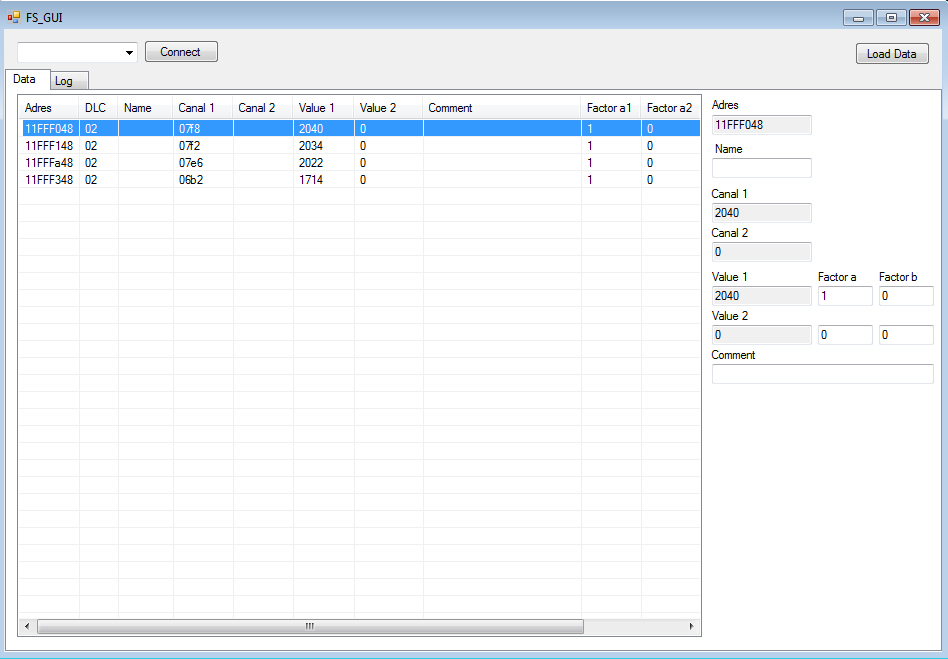
\includegraphics[width=0.65\textwidth]{figures/GUI_Main.PNG}
\caption{G��wne okno programu}
\label{fig:GUI_Main}
\end {figure}

Po uruchomieniu programu pojawia si� okno widoczne na \hyperref[fig:GUI_Main]{Rysunku~\ref*{fig:GUI_Main}}. W g�rnym lewym rogu ekranu znajduje si� rozwijane menu, w kt�rym mo�na wybra� na jakim porcie COM ma by� prowadzony nas�uch. W prawym g�rnym rogu ekranu znajduje si� przycisk $Load Data$, kt�ry umo�liwia wyb�r wczytywania danych w trybie offline. Po nadej�ciu ramki na magistrali lub wczytaniu danych z pliku, w oknie dialogowym pojawia si� informacja z jakich adres�w nadchodzi�y pomiary. Na pozycji Canal widzimy pomiar szesnastkowo, kt�ry zosta� wys�any z uk�adu pomiarowego. Warto�� pozycji Value jest przeskalowana przez wsp�czynniki $a$ i $b$, kt�re domy�lnie s� ustawione na $1$ i $0$. Aplikacja oferuje mo�liwo�� nazwania sygna�u oraz napisania komentarza, co pozwala �atwiej operowa� na przychodz�cych danych. W karcie $Data$ mo�na obserwowa� tylko ostatni� pr�bk�, kt�ra pojawi�a si� na magistrali.\newline

\begin  {figure} 
\centering
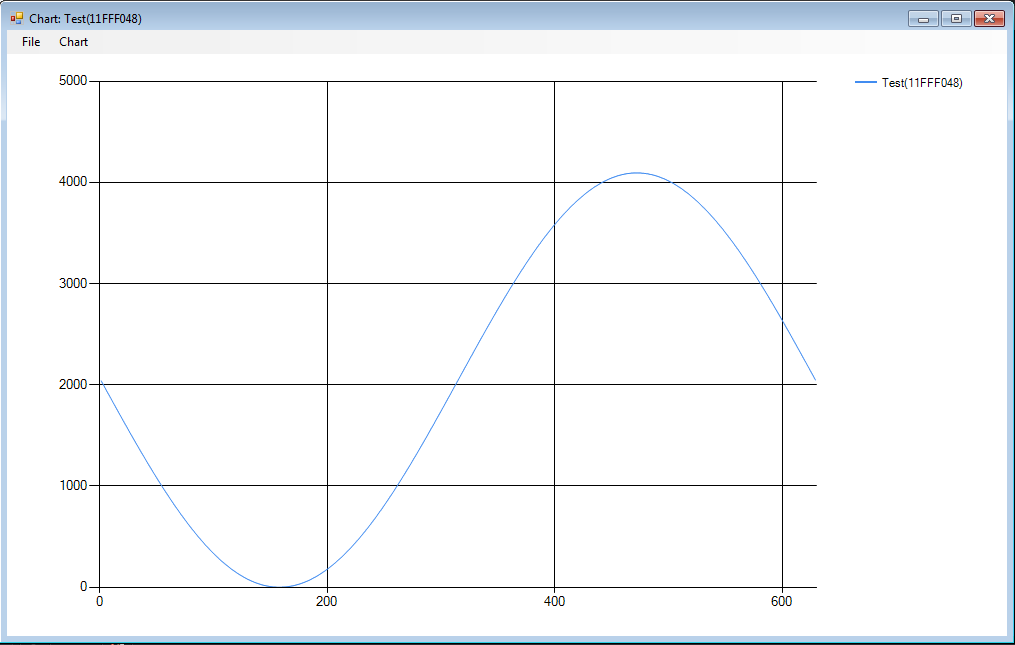
\includegraphics[width=0.65\textwidth]{figures/GUI_Chart.PNG}
\caption{Okno wykresu}
\label{fig:GUI_Chart}
\end {figure}

Dwukrotne klikni�cie na sygna� lub zaznaczenie paru sygna��w i naci�ni�cie klawisza $Enter$, powoduje otwarcie okna z wykresem danego sygna�u, widoczne na \hyperref[fig:GUI_Chart]{Rysunku~\ref*{fig:GUI_Chart}}. W oknie wykresu mo�na obserwowa�, w czasie rzeczywistym lub offline, przebieg sygna�u odczytywanego z magistrali. Przy u�yciu menu rozwijanego $Chart$ mo�na decydowa�, kt�re sygna�y maj� by� obserwowane na wykresie (\hyperref[fig:GUI_Chart]{Rysunek~\ref*{fig:GUI_Menu}}).\newline

\begin  {figure} 
\centering
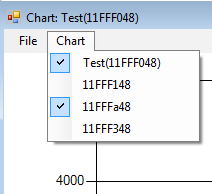
\includegraphics[width=0.3\textwidth]{figures/GUI_Menu.PNG}
\caption{Menu w oknie Chart}
\label{fig:GUI_Menu}
\end {figure}

Menu $File$ w oknie wykresu dostarcza takich opcji jak zapis wykresu do obrazu lub generowanie pliku w formacie obs�ugiwanym przez programy kalkulacyjne.\newline
$GUI$ dostarcza mo�liwo�� pracy na stanowiskach wielomonitorowych. Mo�na otworzy� okno wykresu dla ka�dego kana�u przesy�anego po magistrali $CAN$ i rozmie�ci� je w wygodny dla u�ytkownika spos�b. Przyk�adowe rozmiesczenie okien zaprezentowano na \hyperref[fig:GUI_Charts]{Rysunku~\ref*{fig:GUI_Charts}}.\newline

\begin  {figure} 
\centering
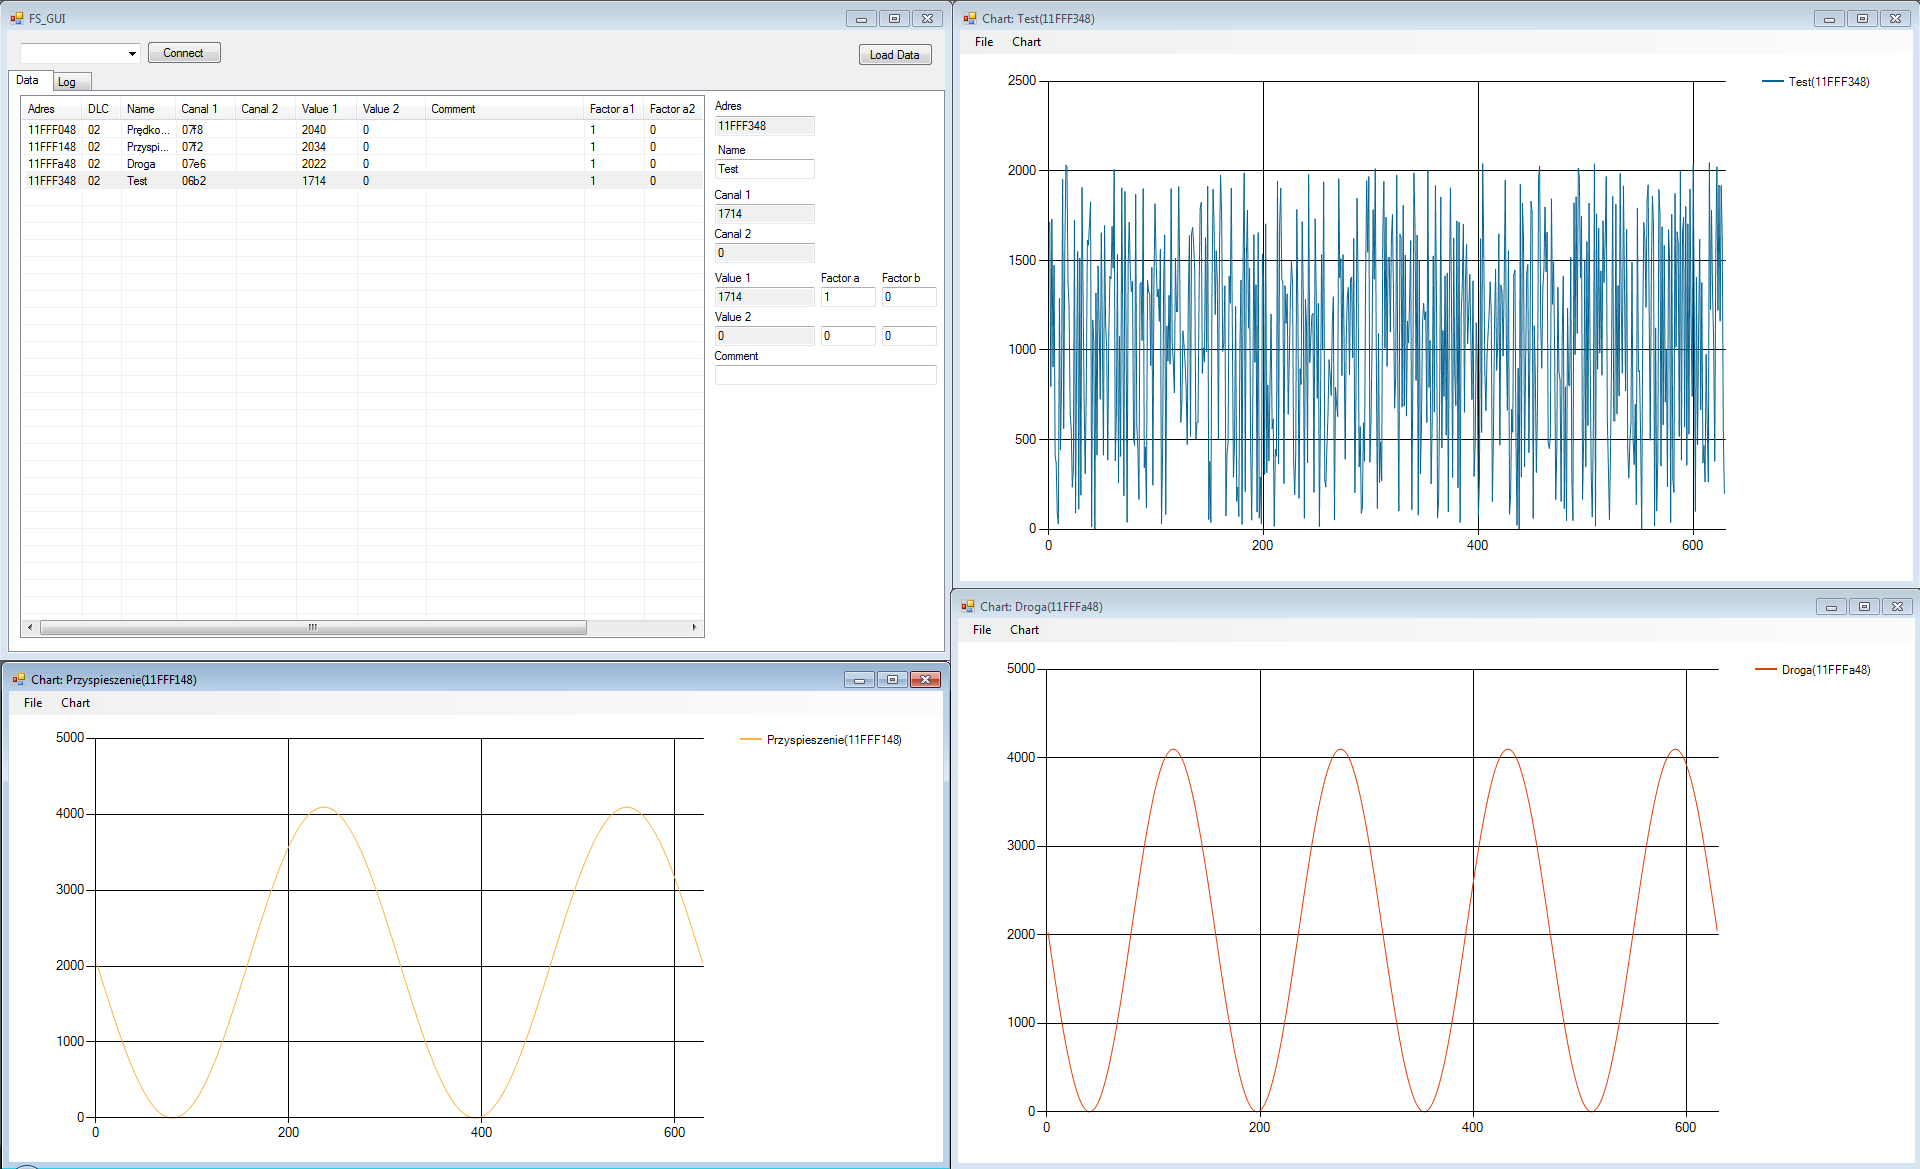
\includegraphics[width=0.8\textwidth]{figures/GUI_All.PNG}
\caption{Praca z wykresami}
\label{fig:GUI_Charts}
\end {figure}

\chapter{Badania eksperymentalne} \label{ch:eksperyment}
\textit{Autorzy: Marcin Aftowicz, Jakub Baranowski}\\ \\

Rozdzia� po�wi�cony jest badaniu dzia�ania systemu. Przedstawiono w nim dow�d na poprawne jego funkcjonowanie oraz na spe�nienie za�o�e� projektowych. Zbadano przebiegi sygna��w i skonfrontowano je z teori�. Por�wnano protoko�y oraz rozwi�zania u�yte w prototypie systemu, z tymi z wersji aktualnej. Pokazano wy�szo�� systemu nad prototypem oraz ograniczenia, kt�re musz� zosta� zlikwidowane w przysz�o�ci.
%=============================================================
%\section{Bank filtr�w akceptacyjnych kontrolera CAN}\label{sec:exp:filtry}
Po otrzymaniu wiadomo�ci na magistrali $CAN$, gdy ta przejdzie przez filtr akceptacyjny, wraz z wiadomo�ci� przechowywana jest informacja o filtrze, kt�ry wiadomo�� dopu�ci� do systemu. Informacja ta zapisana jest w zmiennej $FMI$ (Filter Match Index). Numer filtra nie pokrywa si� jednak z warto�ci� przechowywan� w $FMI$. Podczas inicjalizacji filtr�w, przed uruchomieniem kontrolera $CAN$, nadaje si� ka�demu filtrowi unikalny numer i przypisuje si� go do konkretnej skrzynki odbiorczej FIFO (0 lub 1). Przeprowadzono eksperyment w celu rozwik�ania zagadki numeracji $FMI$ podczas odczytu ramki. Nadano na magistral� $CAN$ wiadomo�ci ze wszystkimi mo�liwymi identyfikatorami wyst�puj�cymi w systemie. W g��wnym komputerze pok�adowym zdefiniowano dwa banki filtr�w akceptacyjnych, przypisuj�c je do dw�ch skrzynek odbiorczych. W \hyperref[tab:FMI]{Tabeli~\ref*{tab:FMI}} przedstawiono odczytane warto�ci $FMI$ wraz z wcze�niej nadanymi numerami filtr�w.

\begin{table}[h]
\caption{Zale�no�� zwr�conej warto�ci $FMI$ od numeracji filtr�w akceptacyjnych}\label{tab:FMI}
\begin{center}
\begin{tabular}{|c|c|c|}
  \hline 
  \cellcolor{gray!50} \textbf{Numer filtru} & \cellcolor{gray!50} \textbf{Numer FIFO} & \cellcolor{gray!50} \textbf{zwr�cone FMI}\\
  \hline
   0 & 0 & 0\\
  \hline
   1 & 0 & 1\\
  \hline
   2 & 0 & 2\\
  \hline
   3 & 0 & 3\\
  \hline
   4 & 0 & 4\\
  \hline
   5 & 0 & 5\\
  \hline
   6 & 0 & 6\\
  \hline \hline
   7 & 1 & 0\\
  \hline 
   8 & 1 & 1\\
  \hline
   9 & 1 & 2\\
  \hline
   10 & 1 & 3\\
  \hline
   11 & 1 & 4\\
  \hline
   12 & 1 & 5\\
  \hline
   13 & 1 & 6\\
  \hline
\end{tabular} 
\end{center}
\end{table}

Wida�, �e numer $FMI$ zale�y od kolejno�ci przyporz�dkowania filtru do konkretnego FIFO, a nie od numeru nadanego podczas inicjalizacji. W przypadku przyporz�dkowania filtr�w od 7 do 13, przyj�y one numery od 0 do 6. Przeprowadzono testy potwierdzaj�ce t� teori�. Przy braku znajomo�ci tej anomalii, u�ytkownicy cz�sto definiuj� w�asne numery filtr�w, pomijaj�c pewne warto�ci i nie mog� zdekodowa� poprawnie ramki. Nast�pstwem jest cz�sto ustawienie maski na warto�� 0x00000000 zapewniaj�cej przyj�cie wszystkich wiadomo�ci, a nast�pnie filtracj� przy u�yciu programu (potwierdzone zachowanie na wielu forach internetowych).\\

Jednym ze sposob�w na omini�cie problemu z�ej numeracji jest zdefiniowanie wszystkich 14 filtr�w w FIFO0. Wtedy warto�� $FMI$ pokryje si� z numerem filtru. Dodatkowo pozostaje kolejne 14 filtr�w, kt�re mo�na przypisa� do FIFO1 i pami�ta� o offsecie r�wnym 14 podczas odczytywania warto�ci $FMI$.

\section{Analiza spe�nienia wymog�w czasowych systemu}\label{sec:exp:timing}
Ilo�� r�nych wiadomo�ci (identyfikator�w w systemie) przedstawionych na \hyperref[fig:adresowanie]{Rysunku~\ref*{fig:adresowanie}} reprezentuje nast�puj�cy wz�r:
\begin{equation}\label{eq:sum_can}
N=\sum_{i=1}^{n} (m_{i})
\end{equation}
gdzie:\\
$N$ - ilo�� r�nych wiadomo�ci\\
$n$ - ilo�� jednostek pomiarowych\\
$m$ - ilo�� wiadomo�ci wysy�anych przez n-t� jednostk� pomiarow�\\

Najkr�tszy czas pr�bkowania poszczeg�lnych wiadomo�ci nie mo�e przekroczy� warto�ci:
\begin{equation}\label{eq:tp}
t_{p_{min}}=N \cdot T
\end{equation}
\begin{equation}\label{eq:T}
T=t_{SD}+t_{UART}
\end{equation}
gdzie:\\
$ t_{p_{min}} $ - minimalny czas pr�bkowania\\
$ N $ - ilo�� r�nych wiadomo�ci\\
$ T $ - czas przetwarzania ramki\\
$ t_{SD} $ - czas zapisu na kart� SD\\
$ t_{UART} $ - czas wys�ania wiadomo�ci przez UART\\

\begin  {figure} [h] 
\centering
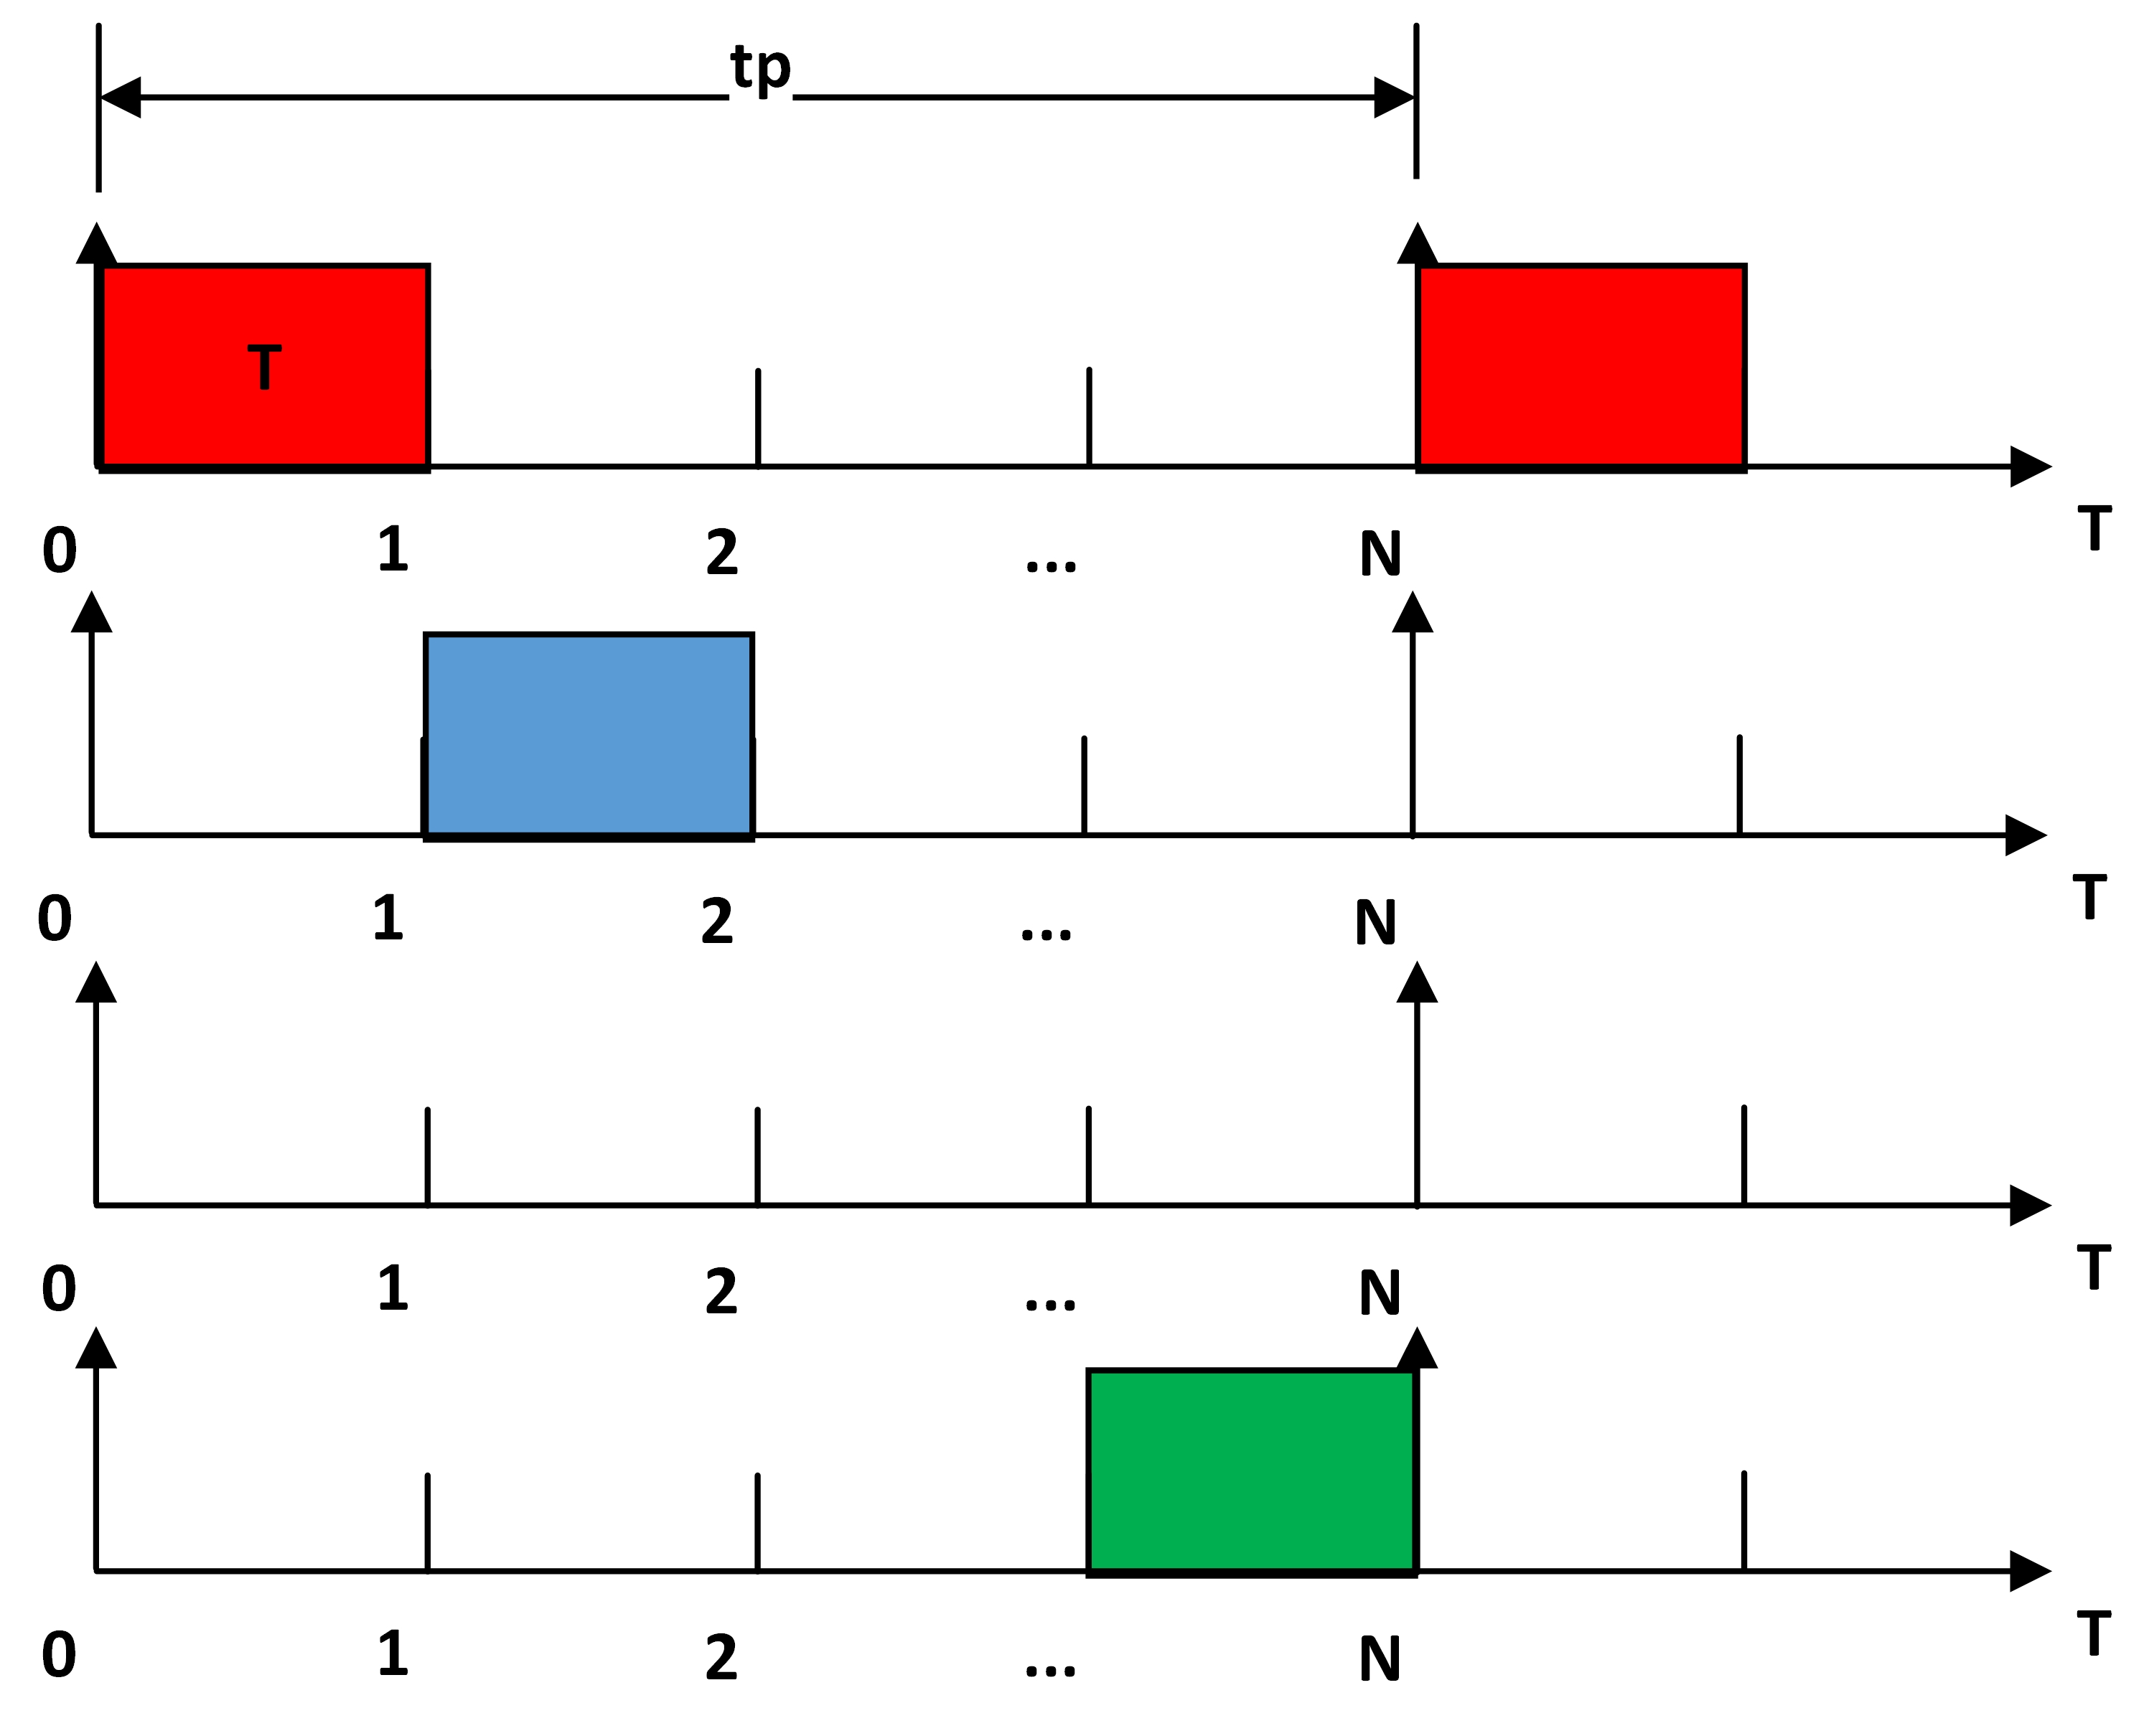
\includegraphics[width=0.6\textwidth]{figures/Gant.JPG}
\caption{Minimalny czas pr�bkowania}
\label{fig:gant}
\end {figure}

Na \hyperref[fig:gant]{Rysunku~\ref*{fig:gant}} przedstawiono diagram Ganta obrazuj�cy minimalny czas pr�bkowania. Przy zbyt cz�stym nadsy�aniu wiadomo�ci, informacje w systemie b�d� gubione.\\

Na podstawie \hyperref[eq:sum_can]{Wzoru~\ref*{eq:sum_can}} obliczono ca�kowit� ilo�� wiadomo�ci w systemie r�wn� 127. Oznacza to, �e czas mi�dzy kolejnymi wiadomo�ciami musi by� 127 razy d�u�szy ni� czas przetwarzania wiadomo�ci. Czas zapisu wiadomo�ci $ t_{SD} $ zmierzono u�ywaj�c wewn�trznego timera. Nie jest to faktyczny czas zapisu, tylko czas, w kt�rym procesor zaanga�owany jest w przesy� danych. Warto�� timera zerowano przed operacj�, a po operacji zapisywano do osobnego pliku. Rezultat przedstawiono na \hyperref[fig:sd_timing]{Rysunku~\ref*{fig:sd_timing}}.

\begin  {figure} [h] 
\centering
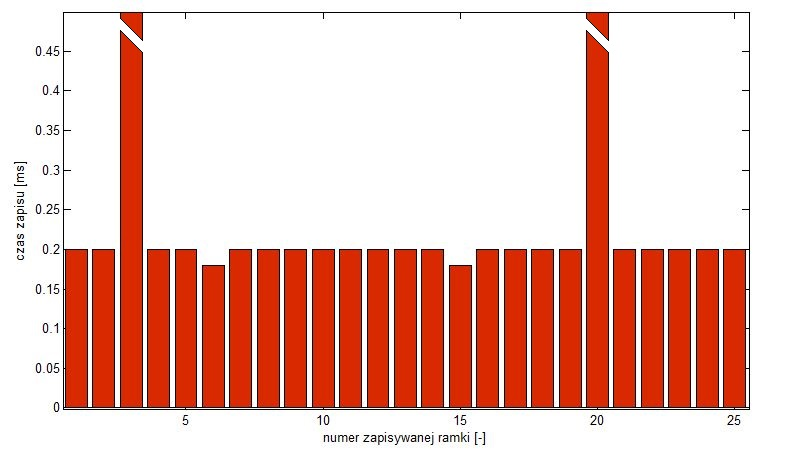
\includegraphics[width=\textwidth]{figures/SD_timing1.JPG}
\caption{Wykres s�upkowy przedstawiaj�cy czas trwania zapisu danych do pliku}
\label{fig:sd_timing}
\end {figure}

Raz na 17 operacji zapisu, czas operacji wykracza� w znacz�cym stopniu poza dopuszczaln� warto��. Czas zapisu wiadomo�ci utrzymywa� si� na poziomie 200 $\mu$s, a w maksimach osi�ga� warto�ci dochodz�ce nawet do 55 ms. D�ugie czasy zapisu wynikaj� z wewn�trznych operacji, kt�re karta wykonuje, zg�aszaj�c stan zaj�to�ci. Aby system funkcjonowa� poprawnie nale�y wprowadzi� bufor, kt�ry przechowuje nadchodz�ce dane w trakcie przerw w zapisie na kart�. Jest to powszechnie znany problem wspominany na forach internetowych. Implementacja buforu to jedna z pierwszych planowanych modernizacji systemu.\\ \\

Czas wysy�ania wiadomo�ci przez UART $ t_{UART} $ zbadano dok�adnie tak samo jak  $ t_{SD} $. Ponownie jest to tylko czas zaj�to�ci procesora. Wynik badania przedstawiono \hyperref[fig:usart_timing]{Rysunku~\ref*{fig:usart_timing}}.

\begin  {figure} [h] 
\centering
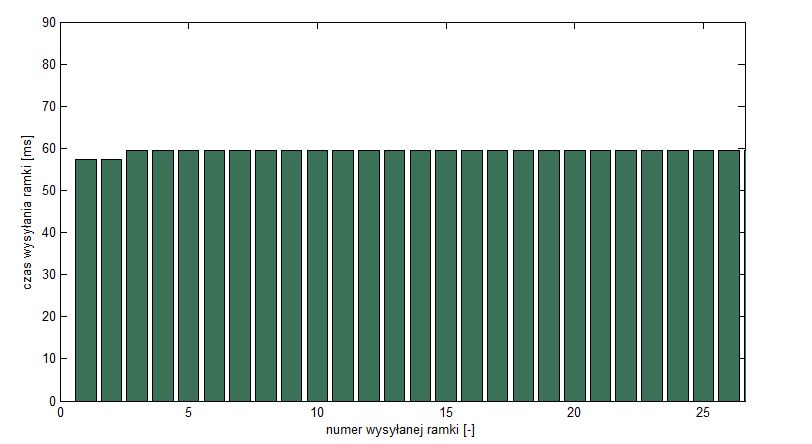
\includegraphics[width=\textwidth]{figures/USART_timing.JPG}
\caption{Wykres s�upkowy przedstawiaj�cy czas wys�ania wiadomo�ci przez UART}
\label{fig:usart_timing}
\end {figure}

W przypadku komunikacji przez UART, bez zaimplementowanej obs�ugi DMA, czas przes�ania wiadomo�ci wynosi oko�o 60 ms. Jest to bardzo du�a warto��, kt�ra musi zosta� zmniejszona aby system m�g� dzia�a� zgodnie z za�o�eniami.\\

Dla aktualnego stanu systemu, chc�c obs�u�y� wszystkie pod��czone w�z�y, wg wzor�w{~\ref{eq:sum_can} i \ref{eq:T}, najkr�tszy mo�liwy czas pr�bkowania wynosi�by:
\begin{equation}
t_{p_{min}}=N \cdot T=127 \cdot (55+60)=14605ms
\end{equation}

Czyli prawie 1,5 s. Chc�c obs�u�y� tylko sterownik silnika w aktualnym stanie systemu, najkr�tszy czas pr�bkowania musia�by wynosi� 805 ms. Po wprowadzeniu bufora, kt�ry zniweluje problem czekania na zapis do pliku, mo�na za�o�y�, �e minimalny czas pr�bkowania zmniejszy�by si� do: 407 ms. Nadal nie jest to satysfakcjonuj�cy wynik.\\

Po wprowadzeniu obs�ugi UART przez kontroler DMA mo�na by uzyska� pr�dko�� wysy�ania danych zbli�on� do pr�dko�ci zapisu do pliku (albo mniejsz�). Wtedy minimalny czas pr�bkowania w systemie prezentowa�by si� nast�puj�co:
\begin{equation}
t_{p_{min}}=N \cdot T=127 \cdot (0,2+0,2)=50.8ms
\end{equation}
50ms  to warto��, kt�ra w pe�ni wystarczy�aby do pr�bkowania szybko-zmiennych proces�w zachodz�cych w poje�dzie. Jest to warto�� u�ywana przez sterownik silnika do pr�bkowania warto�ci takich jak: pr�dko�� obrotowa silnika, po�o�enie przepustnicy (TPS) czy ilo�� tlenu w spalinach (sonda Lambda).\\
Cz�� czujnik�w, na przyk�ad temperatury, nie wymaga tak kr�tkiego czasu pr�bkowania, gdy� zmiana temperatury jest procesem wolno-zmiennym.



\chapter{Podsumowanie}
\textit{Autor: Jakub Baranowski}\\ \\
%=============================================================
%\input{Podsumowanie.tex}


% All appendices and extra material, if you have any.
\cleardoublepage
\appendix%

%\chapter{Rysunki techniczne}
\begin{figure} [h]
\centering
%%----start of first subfigure----
	\subfloat[G�rna warstwa p�ytki]{\label{fig:subfig:front} 
	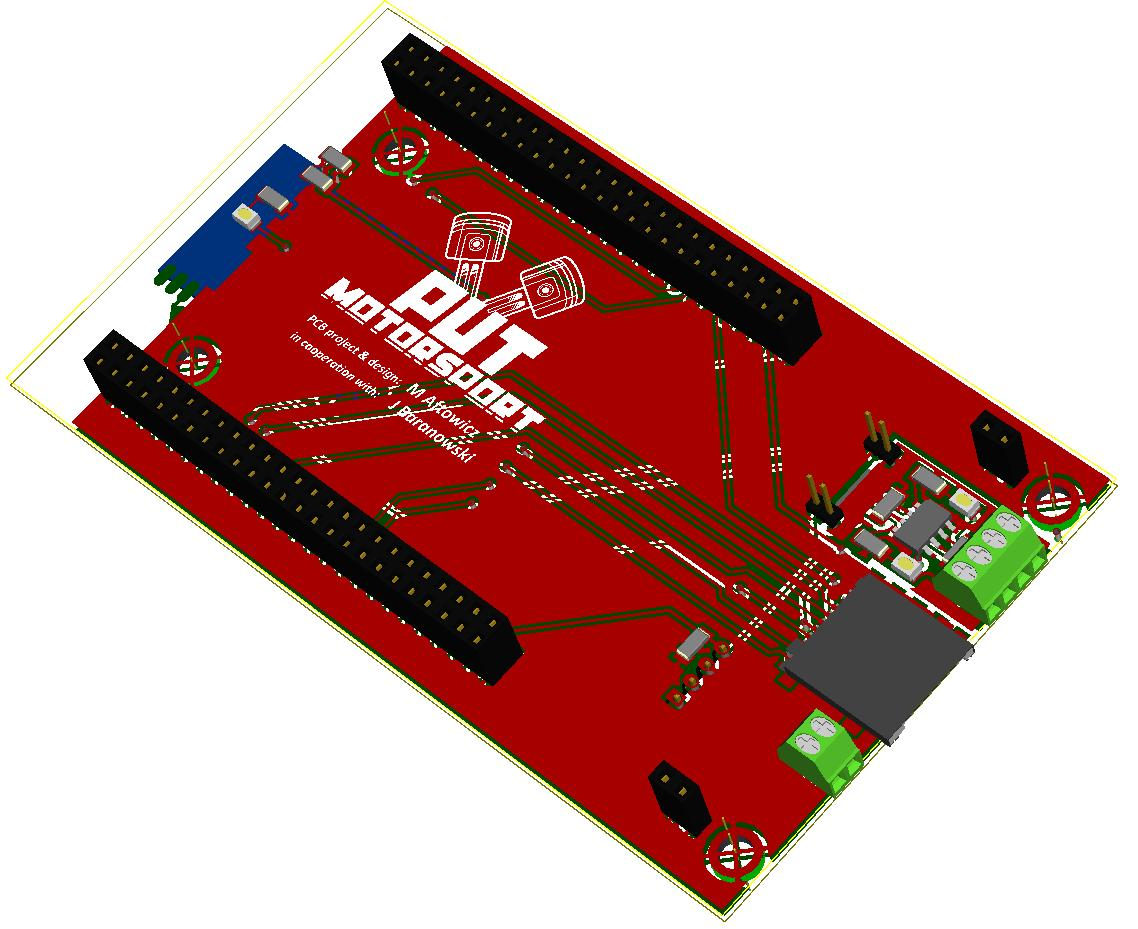
\includegraphics[height=0.3\textheight]{figures/Board_PCB_front.JPG}}
	\hfill
%%----start of second subfigure----
	\subfloat[Dolna warstwa p�ytki]{\label{fig:subfig:back}
	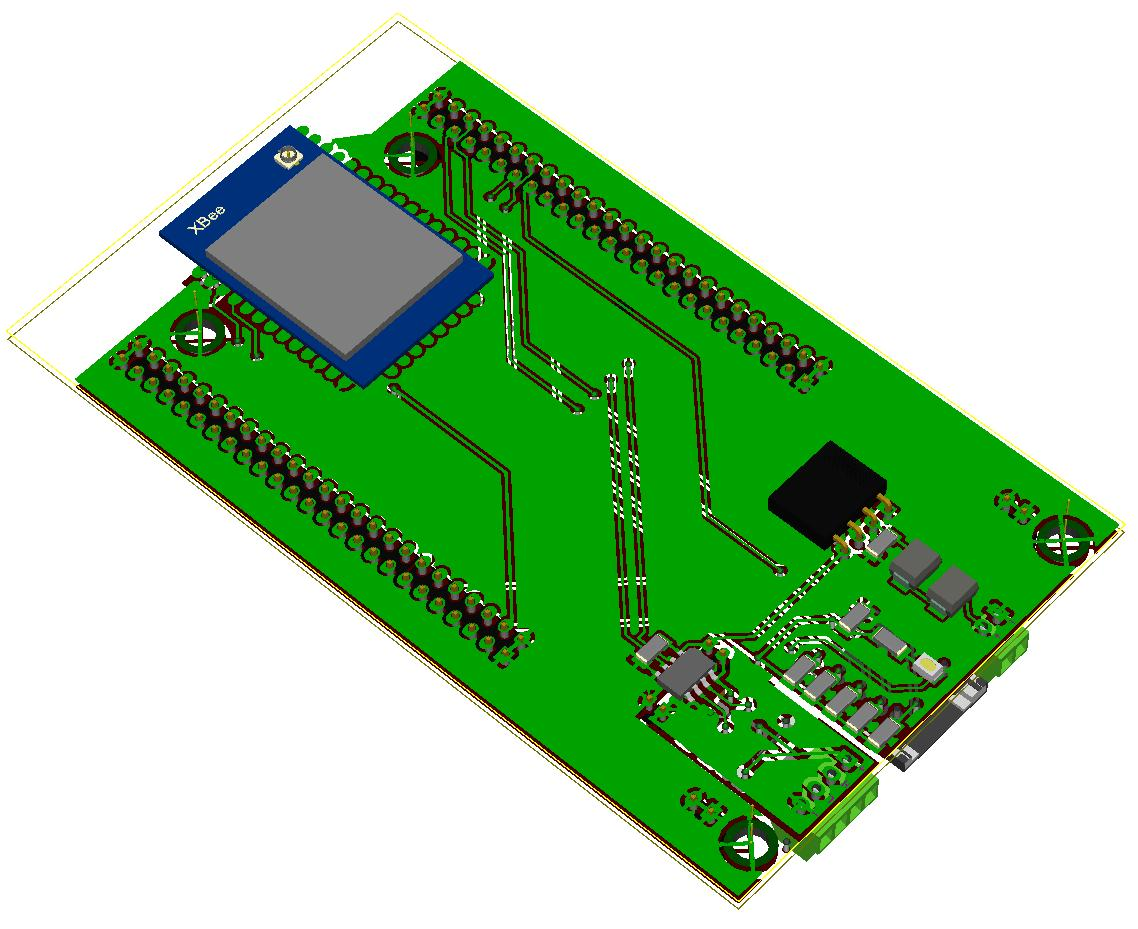
\includegraphics[height=0.3\textheight]{figures/Board_PCB_back.JPG}}
	\caption{Model 3D nak�adki na Discovery}
	\label{fig:3D} %% label for entire figure
\end{figure}

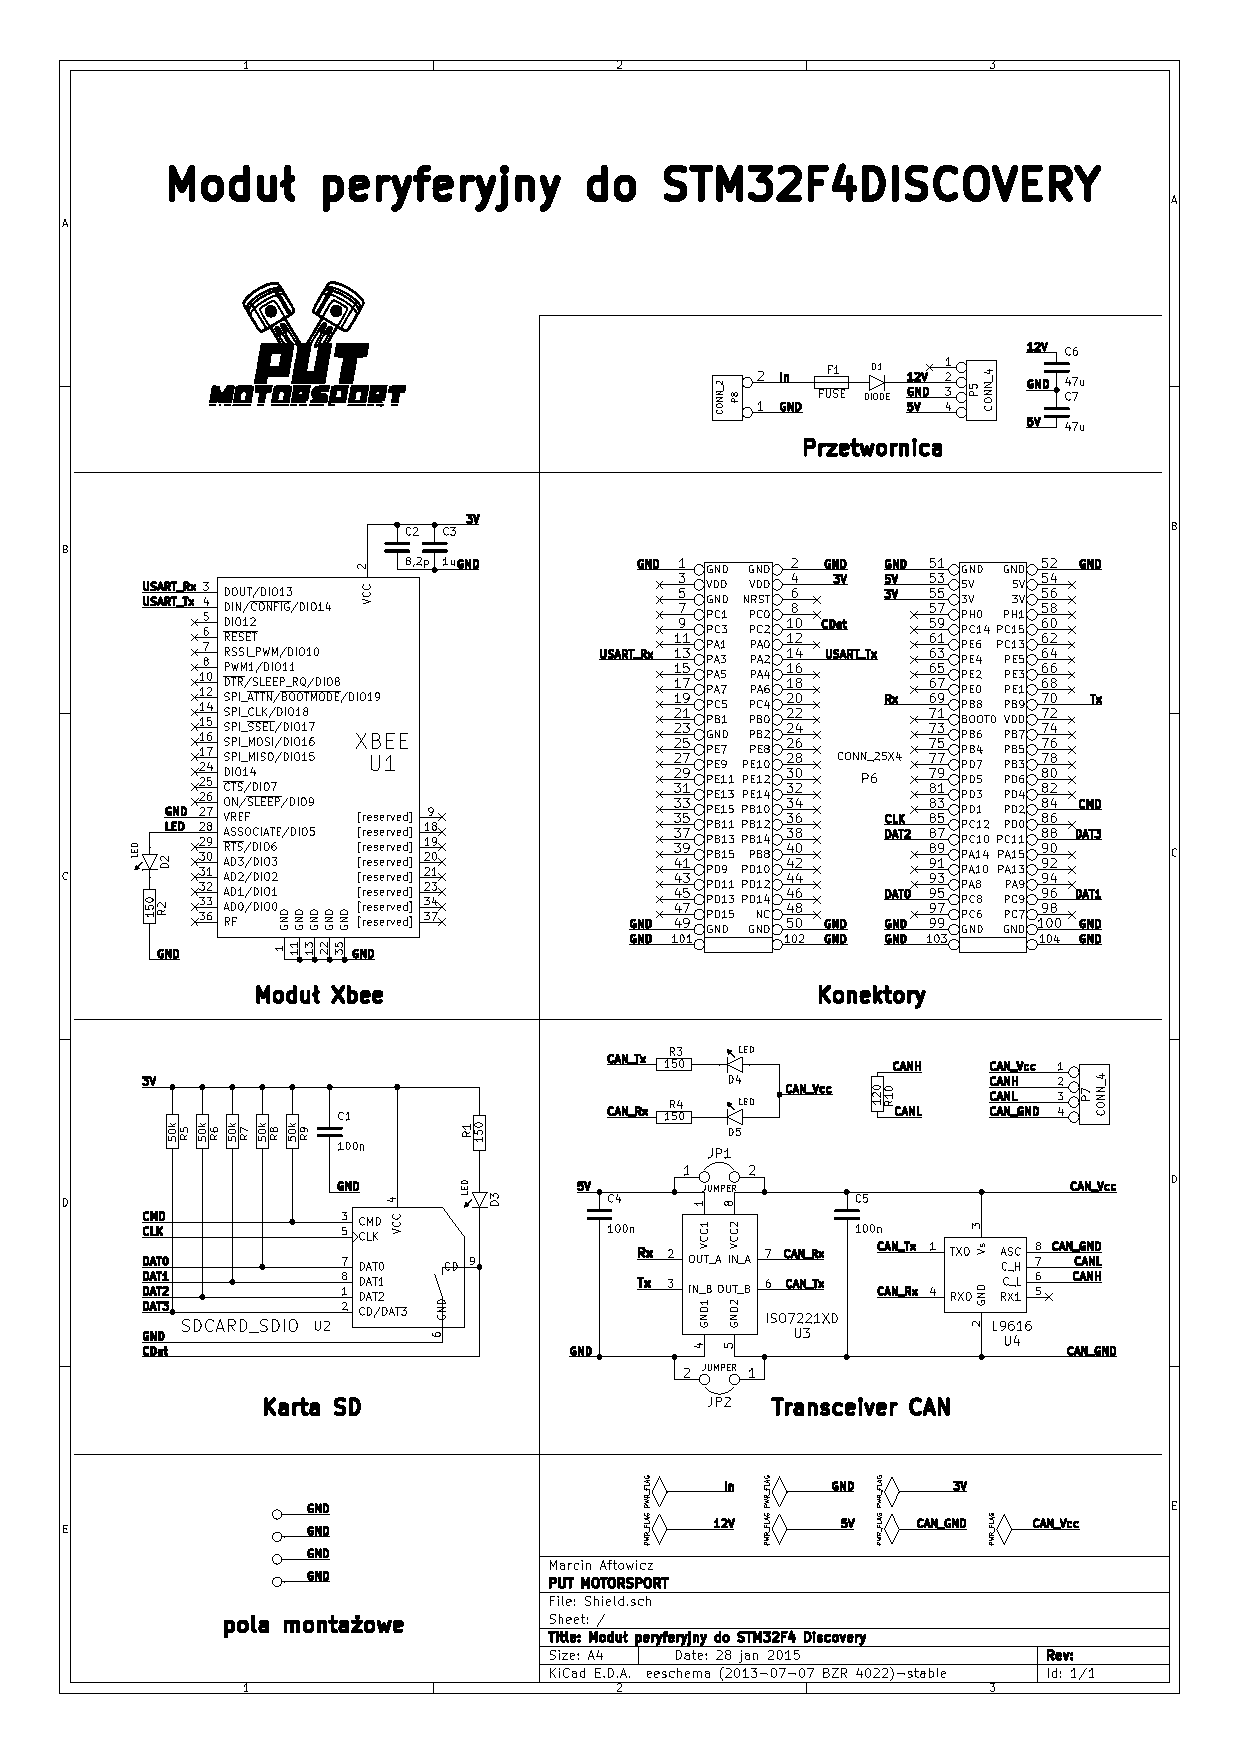
\includepdf[trim=0 0 -1cm 0, pages={1}]{figures/Motherboard_bw.pdf}
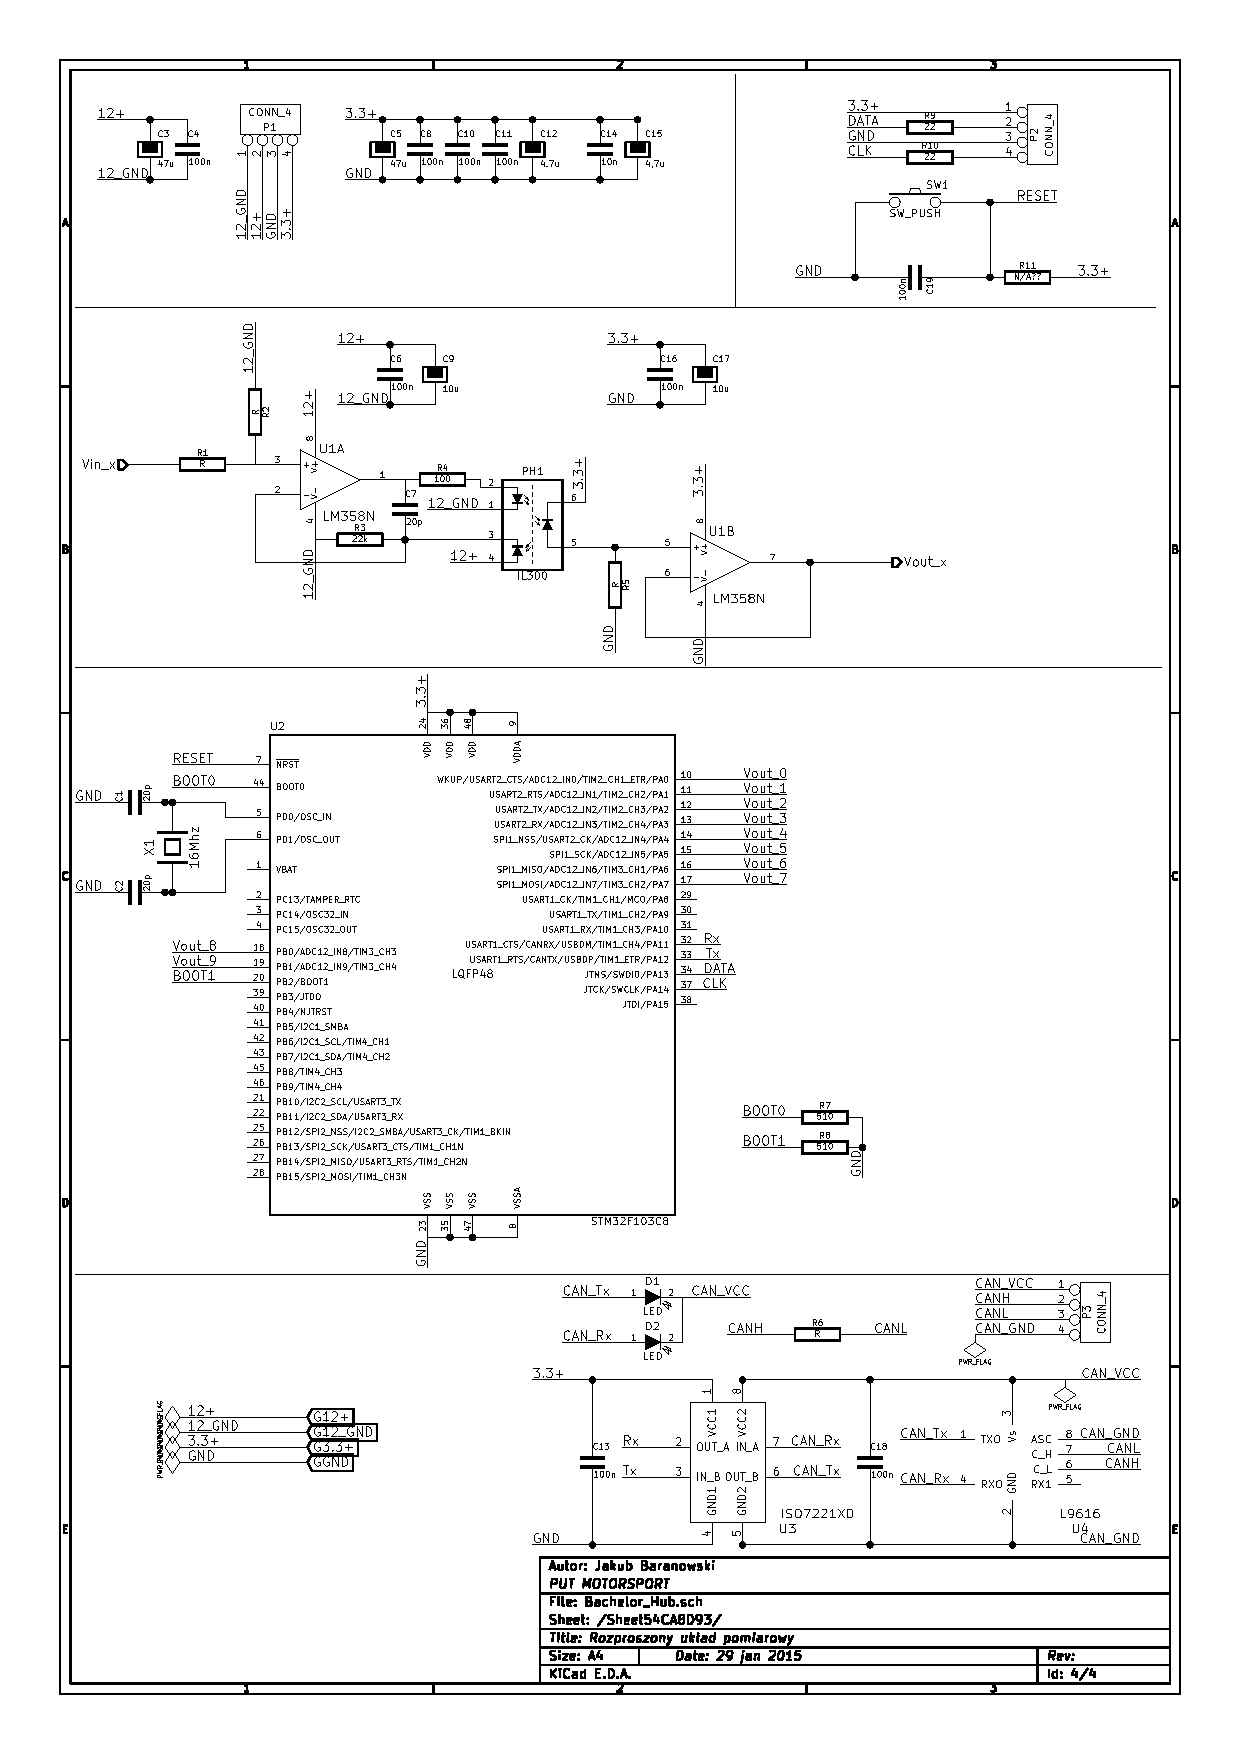
\includepdf[trim=-1cm 0 0 0, pages={1}]{figures/Bachelor_Hub.pdf}
\noindent



%%\input{plyta.tex}
%\cleardoublepage
\hypersetup{ linkcolor={black}}
\cleardoublepage

\bibliography{bibliografia}
\end{document}